% DO NOT COMPILE THIS FILE DIRECTLY!
% This is included by the other .tex files.

\begin{frame}[t,plain]
\titlepage
\end{frame}

\begin{frame}{Structure of the talk}
	\tableofcontents
\end{frame}

%============================================================================
\section{Fundamentos básicos}
%============================================================================

\subsection{Distribuciones}

\begin{frame}{Distribuciones}

\begin{itemize}\itemsep1em
	\item $\Omega\subset\R^d$ open and bounded set.
	\item $\D(\Omega)=\{\varphi\in\mathcal{C}^\infty(\Omega)\colon\varphi\text{ tiene soporte compacto en }\Omega\}$. 
	
	\item \structure{\textbf{Espacio de las distribuciones}}: $\D'(\Omega)$ (espacio dual)
	\begin{itemize}\itemsep1em
		\item $L^p(\Omega)\hookrightarrow\D '(\Omega)$ definida para toda $v\in L^p(\Omega)$ como $\alert{\dualD{v}{\varphi}}=v(\varphi)\coloneqq\int_\Omega v \varphi$, $\forall \varphi\in\D(\Omega)$;
	\end{itemize}

	\item Dada $v\in L^p(\Omega)$ si $g_\alpha=\partial^\alpha v=D^\alpha v\in L^p(\Omega)$ verifica $\dualD{D^\alpha v}{\varphi}=(-1)^{\left|\alpha\right|}\int_\Omega v D^\alpha \varphi$ para todo $\varphi\in\D(\Omega)$ entonces $g_\alpha$ se denomina \structure{\textbf{derivada débil}}.

\end{itemize}
\end{frame}

\subsection{Espacios de Sobolev}
\begin{frame}{Espacios de Sobolev}
Supongamos que $m\in\N\cup\left\{0\right\}$ y $1\leq p\leq+\infty$, $p\in\N$.
\begin{itemize}\itemsep1em
	\item$\displaystyle\alert{W^{m,p}(\Omega)}\coloneqq\{v\in L^p(\Omega):\forall\alpha\in\N^d\mbox{ con }\left|\alpha\right|\leq m, \partial^\alpha v\in L^p(\Omega)\}$
	\begin{itemize}\itemsep1em
		\item Para $p=2$, $\alert{H^{m}(\Omega)}\coloneqq W^{m,2}(\Omega).$
	\end{itemize}
	
	\item Normas definidas $\forall v\in W^{m,p}(\Omega)$:
	\begin{itemize}\itemsep1em
		\item $\displaystyle \alert{\|v\|_{W^{m,p}(\Omega)}}\coloneqq\left(\suma{\substack{\alpha\in\N^d \\ \left|\alpha\right|\leq m}}{}\|\partial^\alpha v\|^p_{L^p(\Omega)}\right)^{1/p}\text{ si }p<+\infty$,
		\item $\displaystyle \alert{\|v\|_{W^{m,\infty}(\Omega)}}\coloneqq\max_{\substack{\alpha\in\N^d \\ \left|\alpha\right|\leq m}}{}\|\partial^\alpha v\|_{L^\infty(\Omega)}\text{ si }p=+\infty$.
	\end{itemize}
	
	\item $\alert{H_0^1(\Omega)}\coloneqq\left\{v\in H^1(\Omega):v_{|_{\partial\Omega}}\equiv 0\right\}$;
	\item $\alert{H(\text{div};\Omega)}\coloneqq\left\{\tau\in(L^2(\Omega))^d\colon\nabla\cdot\tau\in L^2(\Omega) \right\}.$
	
\end{itemize}

\end{frame}

\begin{frame}{Traza}

	\begin{theorem}[Traza]
		
		La aplicación traza
		\begin{align*}
		\alert{\gamma}\colon H^1(\Omega)\cap\mathcal{C}^0(\bar{\Omega})&\to L^2(\partial\Omega)\cap \mathcal{C}(\bar{\partial\Omega})\\
		v	&\mapsto\alert{\gamma(v)}\coloneqq v_{|_{\partial\Omega}}.
		\end{align*}
		se extiende por continuidad a una aplicación lineal y continua de $H^1(\Omega)$ en $L^2(\partial\Omega)$  también llamada $\gamma$.
		
		Existe $C>0$ tal que $\forall v\in H^1(\Omega)$ es $$\norma{\gamma(v)}_{L^2(\partial \Omega)}\leq C\norma{v}_{H^1(\Omega)}.$$
	\end{theorem}
	%\pause
	\textbf{Nota}: generaliza la Fórmula de integración por partes a funciones de $H^1(\Omega)$.
	
\end{frame}

\subsection{Formulación variacional}

\begin{frame}{EDP lineal de orden 2}
\begin{block}{}
\begin{equation*}
\label{ecuacion_general}
\left\{
\begin{aligned}
\mathcal{L}u&=f & \text{en } &\Omega, \\
\mathcal{B}u&=g & \text{en } &\partial\Omega,
\end{aligned}
\right.
\end{equation*}
\end{block}

\begin{itemize}\itemsep1em
\item $\Omega\subset \R^d$ a regular enough open and bounded set (for instance, a polygonal domain).
\item Operador diferencial $\mathcal{L}$ definido para todo $u\colon\Omega\to\R$ como $$\mathcal{L}u=-\nabla\cdot(a\nabla u)+b\nabla u+c u$$ con $a\in [L^\infty(\Omega)]^{d,d}$, $\mathbf{b}\in [L^\infty(\Omega)]^d$ y $c\in L^\infty(\Omega)$.
\item $f\in L^2(\Omega)$.
\item Operador $\mathcal{B}$.
\item $g\colon\Omega\to\R$.
\end{itemize}

\end{frame}

\begin{frame}{Fórmula de integración por partes}
	\textcolor{red}{Cambiar por variacional.}
	\begin{theorem}[Fórmula de integración por partes]
		
		Dadas $u, v\in \mathcal{C}^1(\bar\Omega)$ dos funciones con soporte contenido en $\bar\Omega$, se verifica
		\begin{equation*}
		\label{formula_int_por_partes}
		\int_\Omega u(x)\frac{\partial v}{\partial x_i}(x)dx=-\int_\Omega v(x)\frac{\partial u}{\partial x_i}(x)dx+\int_{\partial \Omega}u(x)v(x)\mathbf{n}_i(x)ds.
		\end{equation*}
		
	\end{theorem}
	
\end{frame}

\begin{frame}{Problema variacional}

\begin{enumerate}
	\item Definir espacio de soluciones $\S\subseteq H^1(\Omega)$  lo suficientemente regular (sentido débil).
	\item \structure{\textbf{Formulación variacional}}: encontrar una función $u\in \S$ que verifique $$a(u,v)=L(v)\text{ para todo }v\in \S.$$
		\begin{itemize}\itemsep1em
			\item $a\colon\S\times\S\to\R$ forma bilineal; 
			\item $L\colon\S\to\R$ forma lineal.
		\end{itemize}
\end{enumerate}

\end{frame}

\begin{frame}{theorem de Lax-Milgram}

\begin{definicion}
	Sea $V$ un espacio de Hilbert y sea $a(\cdot,\cdot):V\times V\longrightarrow\R$ una forma bilineal. Diremos que $a(\cdot,\cdot)$ es \structure{\textbf{coercitiva}} si existe $\nu>0$ tal que $$a(v,v)\geq\nu\norma{v}^2\text{ para todo } v\in V.$$
\end{definicion}

\begin{theorem}[Lax-Milgram]
	\label{theorem:Lax_Milgram}
	Sean $V$ un espacio de Hilbert real, $L(\cdot)$ una forma lineal continua en $V$ y $a(\cdot,\cdot)$ una forma bilineal coercitiva y continua en $V$. La formulación variacional $$a(u,v)=L(v)\text{ para todo }v\in V$$ tiene una única solución $u\in V$ que depende continuamente de la forma lineal $L$.
\end{theorem}

\end{frame}

%-------------------------------
\section{Método de los Elementos Finitos}
%-------------------------------

\subsection{Problema elíptico}

\begin{frame}{Problema elíptico}
Consideramos el problema de Poisson:
\begin{block}{}
\begin{equation*}
\label{prob_modelo_Poisson}
\left\{
\begin{aligned}
-\Delta u&=f & \text{en } &\Omega, \\
u&=0 & \text{en } &\partial\Omega,
\end{aligned}
\right.
\end{equation*}
\end{block}
donde $f\in L^2\left(\Omega\right)$.
\end{frame}

% \subsection{Formulación variacional continua}

\begin{frame}[allowframebreaks]{Formulación variacional continua}

\textbf{Espacio de soluciones}: $\alert{H_0^1(\Omega)}$.
\begin{itemize}\itemsep1em
	\item $a\colon H^1_0(\Omega)\times H_0^1(\Omega)\to\R$, $\displaystyle \alert{a(u,v)}\coloneqq\int_\Omega\nabla u\nabla v$;
	\item $L\colon H_0^1(\Omega)\to\R$, $\displaystyle \alert{L(v)}\coloneqq\int_\Omega f v$.
\end{itemize}
\textbf{Problema variacional}:
\begin{block}{}
	\begin{center}
	\label{form_var_Poisson}
	$\text{encontrar } u\in H^1_0(\Omega) \text{ tal que } a(u,v)=L(v)\text{ para todo } v\in H_0^1(\Omega)$.
	\end{center}
\end{block}
\framebreak
\begin{theorem}
	La forma bilineal $a(\cdot,\cdot)$ es coercitiva y continua.
\end{theorem}

\begin{itemize}\itemsep1em
	\item El problema modelo y su formulación variacional son \alert{equivalentes}.
	\begin{itemize}\itemsep1em
		\item Si $u\in H^2(\Omega)$ es solución del problema modelo $\Rightarrow$ es solución del problema variacional.
		\item Si $u\in H_0^1(\Omega)$ es solución del problema variacional $\Rightarrow$ es solución del problema modelo.
	\end{itemize}
	\item \alert{Lax-Milgram} $\Rightarrow$ existe solución y es única.
\end{itemize}

\end{frame}

\subsubsection{Numerical approximation}

\begin{frame}{Método de Galerkin}
	\begin{block}{}
	\begin{center}
	Elegir $\alert{V_h\subseteq V}$ finito-dimensional con base $\left\{\varphi_i\right\}_{i\in\left\{1,2,\ldots,N_h \right\}}$
	\end{center}
	\end{block}
	
	\vspace*{-0.3cm}
	\begin{itemize}
	\item Encontrar $u\in V$ tal que $a(u,v)=L(v)$ para todo $v\in V$.
	\end{itemize}
	\vspace*{0.1cm}
	$$\Big{\downarrow}$$
	\vspace*{-0.3cm}
	\begin{itemize}
	\item Encontrar $u_h\in V_h$ tal que $a(u_h,v_h)=L(v_h)$ para todo $v_h\in V_h$.
	\end{itemize}
	\vspace*{0.1cm}
	$$\Big{\Updownarrow}$$
	\vspace*{-0.3cm}
	\begin{itemize}
	\item Resolver el sistema lineal $A\mathbf{U}=\mathbf{F}$ donde:
	\vspace*{0.3cm}
	\begin{itemize}
		\item $A=\left(A_{i j}\right)_{i, j\in\left\{1,2,\ldots,N_h\right\}}$ con $A_{i j}=a(\varphi_j,\varphi_i)$;
		\item $\mathbf{U}=\left(U_1,U_2,\ldots,U_{N_h}\right)^t$ con $u_h=\displaystyle\sum_{i=1}^{N_h}U_i\varphi_i$;
		\item $\mathbf{F}=\left(F_1,F_2,\ldots,F_{N_h}\right)^t$ con $F_i=L\left(\varphi_i\right)$.
	\end{itemize}
	\end{itemize}
\end{frame}
	
% \begin{frame}{Cota de error}
% 	\begin{lemma}
% 		Supongamos que $a(\cdot,\cdot)$ es coercitiva y continua. Se verifica que
% 		\begin{equation*}
% 		\norma{u-u_h}\leq \frac{M}{\nu} \inf_{v_h\in V_h}\norma{u-v_h}
% 		\end{equation*}
% 		donde $M>0$ y $\nu>0$ son las constantes de continuidad y coercitividad, respectivamente, de $a(\cdot,\cdot)$.
% 	\end{lemma}
	
% \end{frame}

\begin{frame}{Elemento finito unisolvente}

\begin{definicion}
	Denominamos \structure{\textbf{elemento finito unisolvente}} a la terna $\alert{\left(K,\mathcal{P},\Sigma\right)}$ donde
	\begin{itemize}
		\item $K\subseteq \R^d$ es un compacto con interior no vacío y frontera de Lipschitz;
		\item $\mathcal{P}$ es un espacio de funciones $p\colon K\longrightarrow\R$ finito-dimensional de dimensión $N_\mathcal{P}$;
		\item $\Sigma=\left\{\sigma_1,\sigma_2,\ldots,\sigma_{N_\mathcal{P}}\right\}\subseteq\mathcal{L}\left(\mathcal{P},\R\right)$ es tal que
		\begin{align*}
		\sigma\colon\mathcal{P}&\longrightarrow \R^{N_\mathcal{P}}\\
		p&\longmapsto \left(\sigma_1(p),\sigma_2(p),\ldots,\sigma_{N_\mathcal{P}}(p)\right)
		\end{align*}
		es biyectiva.
	\end{itemize}
\end{definicion}

\end{frame}

\begin{frame}{Malla de $\bar{\Omega}$}

\begin{definicion}
	Una \structure{\textbf{malla}} de $\bar{\Omega}$ es un conjunto $\alert{\mathcal{T}_h}$ de $d$-símplices $\left(K_i\right)_{i\in\left\{1,2,\ldots,N_{\mathcal{T}_h}\right\}}$ no degenerados que satisfacen:
	\begin{itemize}
		\item $K_i\subseteq\bar\Omega$ para todo $i\in\left\{1,2,\ldots,N_{\mathcal{T}_h}\right\}$;
		\item $\text{int}\left(K_i\right)\cap\text{int}\left(K_j\right)=\varnothing$ para $i,j\in\left\{1,2,\ldots,N_{\mathcal{T}_h} \right\}$ con $i\neq j$;
		\item $\displaystyle \bigcup_{i=1}^{N_{\mathcal{T}_h}} K_i=\bar\Omega$.
	\end{itemize}	
	La malla es \structure{\textbf{conforme}} si además verifica que:
	\begin{itemize}
		\item $K_i\cap K_j$ para $i,j\in\left\{1,2,\ldots,N_{\mathcal{T}_h} \right\}$ con $i\neq j$ es un $m$-símplice con $m\in\left\{0,1,\ldots,d-1 \right\}$ cuyos vértices son también de $K_i$ y $K_j$.
	\end{itemize}
\end{definicion}

\end{frame}

\begin{frame}{Elementos finitos de Lagrange}
	\scriptsize
\begin{definicion}
	Sea $\left(K,\mathcal{P},\Sigma\right)$ un elemento finito unisolvente. Si existen un conjunto de puntos $\{a_1,a_2,\ldots,a_{N_\mathcal{P}}\}\subset K$ tales que para todo $p\in\mathcal{P}$ se verifica que $$\sigma_i(p)=p(a_i)\quad\text{para todo}\quad i\in\{1,2,\ldots,N_{\mathcal{P}}\},$$ llamamos a la terna $\alert{\left(K,\mathcal{P},\Sigma\right)}$ \structure{\textbf{elemento finito de Lagrange}}.
	
	Los puntos $\{a_1,a_2,\ldots,a_{N_\mathcal{P}}\}$ de llaman \structure{\textbf{nodos del elemento finito}} y la base de Lagrange definida como $$B_L\coloneqq\left\{L_i\in\mathbb{P}_k\colon L_i(a_j)=\delta_{ij}\quad\forall i,j\in\{1,2,\ldots,N_\mathcal{P}\} \right\}$$ se denomina \structure{\textbf{base nodal}} de $\mathcal{P}$.
\end{definicion}
En la práctica: \structure{\textbf{elementos finitos simpliciales de Lagrange}}.

\begin{block}{}
	\begin{center}
	$V_h=\left\{v_h\in \mathcal{C}^0\left(\bar\Omega\right)\colon v_{h|_{K_i}}\in \mathcal{P}_i \text{ con } K_i\in\mathcal{T}_h, \forall i\in\left\{1,2,\ldots,N_{\mathcal{T}_h} \right\}\right\}$
	\end{center}
	\end{block}
	
	
	Generalmente $\mathcal{P}_i=\mathbb{P}_k(K_i)$.
\end{frame}

\begin{frame}{Error analysis}
	\begin{block}{}
		\begin{center}
		$V_h=\left\{v_h\in \mathcal{C}^0\left(\bar\Omega\right)\colon v_{h|_{K_i}}\in \mathbb{P}_k(K_i) \text{ con } K_i\in\mathcal{T}_h, \forall i\in\left\{1,2,\ldots,N_{\mathcal{T}_h} \right\}\right\}$
		\end{center}
	\end{block}

	\vspace*{1cm}
	\begin{theorem}
		If $u\in H^s(\Omega)$ with $\frac{d}{2}<s\le k+1$, there exists $c_1,c_2>0$ such that
		\begin{align*}
			\norma{u-u_h}_{H^1(\Omega)}&\le c_1 h^{s-1}\norma{u}_{H^s(\Omega)},\\
			\norma{u-u_h}_{L^2(\Omega)}&\le c_2 h^{s}\norma{u}_{H^s(\Omega)}.
		\end{align*}
	\end{theorem}
\end{frame}

\subsubsection{Numerical experiments}

\subsection{Hyperbolic problem}

\begin{frame}{Problema modelo}
	Consideramos el problema de convección-reacción:
	\begin{block}{}
	\begin{equation*}
	\label{prob_modelo_hiperbolica}
	\left\{
	\begin{aligned}
	\beta\cdot\nabla u+\mu u&=f & \text{en } &\Omega, \\
	u&=0 & \text{en } &\partial\Omega^-,
	\end{aligned}
	\right.
	\end{equation*}
	\end{block}
	donde 
	\begin{itemize}
		\item $\partial\Omega^-=\left\{x\in\partial\Omega\colon \beta(x)\mathbf{n}(x)<0\right\},$
		\item $\mu\in L^\infty(\Omega)$,
		\item $\beta\in\left[\text{Lip}(\Omega)\right]^d$,
		\item $f\in L^2(\Omega)$.
	\end{itemize}
	\vspace*{.5cm}
	Asumimos que existe $\mu_0>0$ tal que $\displaystyle\mu-\frac{1}{2}\nabla\cdot\beta\geq\mu_0$ en $\Omega$.
	
	\end{frame}
	
	\begin{frame}{Espacio de los grafos}
	
	\begin{definicion}
	Se define el \structure{\textbf{espacio de los grafos}} como $$\alert{V}\coloneqq\left\{v\in L^2(\Omega)\colon\beta\cdot\nabla v\in L^2(\Omega) \right\},$$
	which is a Hilbert space with the norm:
	$$
	\norma{v}_V=\sqrt{\norma{v}_{L^2(\Omega)}^2+\norma{\beta\cdot\nabla v}_{L^2(\Omega)^d}}^2.
	$$
	\end{definicion}
	
	\begin{definicion}
	Se define el \structure{\textbf{espacio de Lebesgue con peso}} $$\alert{L^2(|\beta\cdot\mathbf{n}|;\partial\Omega)}\coloneqq\left\{v\text{ es medible en }\Omega\colon\int_{\partial\Omega}|\beta\cdot\mathbf{n}|v^2<\infty \right\}$$ y la norma $\forall v\in L^2(|\beta\cdot\mathbf{n}|;\partial\Omega)$ como $$\alert{\norma{v}_{L^2(|\beta\cdot\mathbf{n}|;\partial\Omega)}}\coloneqq\norma{\sqrt{|\beta\cdot\mathbf{n}|}v}_{L^2(\partial\Omega)}.$$
	\end{definicion}
	\end{frame}
	\begin{frame}{Trazas e integración por partes}
	\begin{lemma}[Trazas e integración por partes]
	La aplicación traza
	\begin{align*}
	\alert{\gamma}\colon {C}^0(\bar{\Omega})&\to L^2(|\beta\cdot\mathbf{n}|;\partial\Omega)\\
	v	&\mapsto\alert{\gamma(v)}\coloneqq v_{|_{\partial\Omega}}.
	\end{align*}
	se extiende por continuidad a $V$.
	 
	Existe una constante $C>0$ tal que $\forall v\in V$ tenemos que $$\norma{\gamma(v)}_{L^2(|\beta\cdot\mathbf{n}|;\partial \Omega)}\leq C\norma{v}_V.$$
	
	Se verifica $\forall v,w\in V$ la siguiente fórmula de integración por partes: $$\int_\Omega\left[(\beta\cdot\nabla v)w+(\beta\cdot\nabla w)v+(\nabla\cdot\beta)vw\right]=\int_{\partial\Omega}(\beta\cdot \mathbf{n})\gamma(v)\gamma(w).$$
	\end{lemma}
	
	\end{frame}
	
	\begin{frame}{Formulación variacional continua}
	\textbf{Espacio de soluciones}: $\alert{V}$ (espacio de los grafos).
	\begin{itemize}\itemsep1em
		\item $a\colon V\times V\to \R$, $$\alert{a(u,v)}\coloneqq\int_\Omega(\beta\cdot\nabla u)v+\int_\Omega\mu u v+\int_{\partial\Omega}(\beta\mathbf{n})^-uv;$$
		\item $L\colon V\to\R$, $$\alert{L(v)}\coloneqq\int_\Omega f v.$$
	\end{itemize}
	\textbf{Problema variacional}:
	\begin{block}{}
		\begin{center}
			$\text{encontrar }u\in V\text{ tal que }a(u,v)=L(v)\text{ para todo } v\in V.$
		\end{center}
	\end{block}
	
	\begin{itemize}\itemsep1em
		\item In this case, $a(\cdot,\cdot)$ is \alert{not coercive in $V$}.
		\item El problema modelo y su formulación variacional son \alert{equivalentes} en $V$.
		\item Existe solución y es única.
	\end{itemize}
	
	\end{frame}

\subsubsection{Numerical approximation}

\begin{frame}{Método de Galerkin}
	\begin{block}{}
	\begin{center}
	Elegir $\alert{V_h\subseteq V}$ finito-dimensional con base $\left\{\varphi_i\right\}_{i\in\left\{1,2,\ldots,N_h \right\}}$
	\end{center}
	\end{block}
	
	\vspace*{-0.3cm}
	\begin{itemize}
	\item Encontrar $u\in V$ tal que $a(u,v)=L(v)$ para todo $v\in V$.
	\end{itemize}
	\vspace*{0.1cm}
	$$\Big{\downarrow}$$
	\vspace*{-0.3cm}
	\begin{itemize}
	\item Encontrar $u_h\in V_h$ tal que $a(u_h,v_h)=L(v_h)$ para todo $v_h\in V_h$.
	\end{itemize}
	\vspace*{0.1cm}
	$$\Big{\Updownarrow}$$
	\vspace*{-0.3cm}
	\begin{itemize}
	\item Resolver el sistema lineal $A\mathbf{U}=\mathbf{F}$ donde:
	\vspace*{0.3cm}
	\begin{itemize}
		\item $A=\left(A_{i j}\right)_{i, j\in\left\{1,2,\ldots,N_h\right\}}$ con $A_{i j}=a(\varphi_j,\varphi_i)$;
		\item $\mathbf{U}=\left(U_1,U_2,\ldots,U_{N_h}\right)^t$ con $u_h=\displaystyle\sum_{i=1}^{N_h}U_i\varphi_i$;
		\item $\mathbf{F}=\left(F_1,F_2,\ldots,F_{N_h}\right)^t$ con $F_i=L\left(\varphi_i\right)$.
	\end{itemize}
	\end{itemize}
\end{frame}

\begin{frame}{Error analysis}
	\begin{block}{}
		In this case, the-non coercitivity of $a(\cdot,\cdot)$ implies that, in general, we cannot have error estimates of the type:
		$$
		\norma{u-u_h}_V\le c h^s,
		$$
		for some $c,s>0$.

		\vspace*{1cm}
		$\Longrightarrow$ \alert{The error may not decrease!!}
	\end{block}
\end{frame}

\subsubsection{Numerical experiments}

\section{Discontinuous Galerkin methods}

	\subsection{Elliptic problem}

	\begin{frame}{Problema elíptico}
		Consideramos el problema de Poisson:
		\begin{block}{}
		\begin{equation*}
		\label{prob_modelo_Poisson}
		\left\{
		\begin{aligned}
		-\Delta u&=f & \text{en } &\Omega, \\
		u&=0 & \text{en } &\partial\Omega,
		\end{aligned}
		\right.
		\end{equation*}
		\end{block}
		donde $f\in L^2\left(\Omega\right)$.
		\end{frame}

	\subsubsection{Numerical approximation}

\begin{frame}[allowframebreaks]{Espacios de Sobolev rotos}
\begin{definicion}
	Definimos para $m\in\N\cup\{0\}$ y $1\leq p\leq+\infty$ el \structure{\textbf{espacio de Sobolev roto}}
	$$\alert{W^{m,p}(\T_h)}\coloneqq\left\{v\in L^p(\Omega)\colon \forall K\in\T_h, v_{|_K}\in W^{m,p}(K)\right\}$$
	con la norma
	$\displaystyle\alert{\norma{v}_{W^{m,p}(\T_h)}}\coloneqq\left(\sum_{K\in\T_h} \norma{v}^p_{W^{m,p}(K)}\right)^{1/p}.$
	Asimismo, se define el espacio
	$$\alert{H^m(\mathcal{T}_h)}\coloneqq W^{m,2}(\T_h)= \left\{v\in L^2(\Omega)\colon \forall K\in\T_h, v_{|_K}\in H^m(K) \right\}$$
	con la norma
	$\displaystyle\alert{\norma{v}_{H^m(\T_h)}}\coloneqq \left(\sum_{K\in\T_h}\norma{v}^2_{H^m(K)} \right)^{1/2}.$
\end{definicion}
\framebreak
\begin{definicion}
	El \structure{\textbf{gradiente roto}} $\nabla_h\colon H^1(\T_h)\to (L^2(\Omega))^d$ se define tal que $\forall v\in H^1(\T_h)$, $$\alert{(\nabla_h v)_{|_T}}\coloneqq\nabla(v_{|_T})\text{ para todo } T\in\T_h.$$
\end{definicion}

\begin{lemma}
	\label{lemma:inclusion_sobolev}
	Sea $m\in\N\cup\{0\}$ y sea $1\leq p\leq+\infty$. Se tiene que $\alert{W^{m,p}(\Omega)\subset W^{m,p}(\T_h)}$. Más aún, para todo $v\in W^{1,p}(\Omega)$ se verifica que $\nabla_h v=\nabla v$ en $\left(L^p(\Omega)\right)^d$.
\end{lemma}
\end{frame}

\begin{frame}{Otro espacio roto}
\begin{definicion}
	Se define el espacio roto $$\alert{H(\text{div};\T_h)}\coloneqq\left\{\tau\in(L^2(\Omega))^d\colon \forall T\in\T_h, \tau_{|_T}\in H(\text{div};T)\right\}$$ y el \structure{\textbf{operador divergencia roto}} $\nabla_h\cdot\colon H(\text{div};\T_h)\to L^2(\Omega)$ tal que para todo $\tau\in H(\text{div};\T_h)$ se tiene que $$(\nabla_h\cdot\tau)_{|_T}\coloneqq \nabla\cdot(\tau_{|_T})\text{ para todo }T\in\T_h.$$
\end{definicion}

\end{frame}

\begin{frame}{Saltos y medias}
\begin{itemize}
	\item $\alert{\E_h^i}\subset\Omega$ es el conjunto de los $(d-1)$-símplices interiores a la malla $\T_h$;
	\item $\alert{\E_h^b}\subset\partial\Omega$ es el conjunto de los $(d-1)$-símplices en la frontera de la malla $\T_h$.
\end{itemize}

\begin{definicion}
	Sean $K_1,K_2\in\T_h$ dos elementos de la malla.
	
	\begin{itemize}
		\item Si $e=K_1\cap K_2\in \E_h^i$ definimos para todo $v\in H^m(\T_h)$ con $m\in\N$
		
		\begin{itemize}\itemsep1em
			\item \structure{\textbf{salto}}: $\alert{\salto{v}_e}\coloneqq v_{|_{K_1^e}}-v_{|_{K_{2}^e}}$;
			\item \structure{\textbf{media}}: $\alert{\media{v}_e}\coloneqq \dfrac{1}{2}\left(v_{|_{K_1^e}}+v_{|_{K_{2}^e}}\right) $.
		\end{itemize}
		
		\item Si $e=K_1\cap \partial\Omega\in \E_h^b$ definimos para todo $v\in H^m(\T_h)$ con $m\in\N$
		
		\begin{itemize}\itemsep1em
			\item \structure{\textbf{salto}}: $\alert{\salto{v}_e}\coloneqq v_{|_{K_1^e}}$;
			\item \structure{\textbf{media}}: $\alert{\media{v}_e}\coloneqq v_{|_{K_1^e}}$.
		\end{itemize}
		
	\end{itemize}
	
\end{definicion}
\end{frame}

\begin{frame}{Caracterización de espacios de Sobolev}

\begin{lemma}[Caracterización de $W^{1,p}(\Omega)$]
	\label{lemma:caracterizacion_sobolev}
	Sea $1\leq p\leq \infty$. Una función $v\in W^{1,p}(\T_h)$ pertenece a $W^{1,p}(\Omega)$ si y sólo si $\salto{v}=0$ para todo $e\in\E_h^i$.
\end{lemma}

\begin{lemma}[Caracterización de $H(\text{div};\Omega)$]
	Una función $\tau\in H(\text{div};\T_h)\cap \left[W^{1,1}(\T_h)\right]^d$ pertenece a $H(\text{div};\Omega)$ si y solo si $\salto{\tau\cdot\mathbf{n}_e}=0$ para todo $e\in\E_h^i$.
\end{lemma}

\end{frame}

\begin{frame}{Espacio finito-dimensional}
\textbf{Espacio finito dimensional}:$$\alert{\mathbb{P}_k^d(\T_h)}\coloneqq\left\{v_h\in L^2(\Omega)\colon v_{h|_{K_i}}\in\mathbb{P}_k(K_i)\text{ con } K_i\in\T_h,\forall i\in\left\{1,2,\ldots,N_{\T_h}\right\}\right\}$$ con base $\left\{\phi_i\right\}_{i=1}^{N_h^{\text{sip}}}$.
\vspace*{1cm}

Denotamos
\begin{itemize}\itemsep1em
\item $\S_h\coloneqq\mathbb{P}_k^d(\T_h)$,
\item $\S_{*h}\coloneqq H^1_0(\Omega)\cap H^2(\Omega)+\S_h$.
\end{itemize}
\vspace*{1cm}
\pause
$\alert{\mathbb{P}_k^d(\T_h)\not\subset H_0^1(\Omega)}$ (espacio no conforme \alert{!!})
\end{frame}

\begin{frame}{Método de Penalización Interior Simétrico}
\begin{itemize}\itemsep1em
	\item $a_h^{\text{sip}}:\S_{*h}\times \S_h\to\R$,
	\begin{equation*}
	\label{forma_bilineal_DG}
	\begin{aligned}
	\alert{\asip{u}{v_h}}&\coloneqq \framedmath<2>{\displaystyle \sum_{K\in\T_h}\int_K\nabla_h u\nabla_h v-\sum_{e\in\E_h}\int_e\media{\nabla_h u\cdot\mathbf{n}_e}\salto{v_h}}\\&\framedmath<3>{\displaystyle -\sum_{e\in\E_h}\int_e\media{\nabla_h v\cdot\mathbf{n}_e}\salto{u}}\\&\framedmath<4>{\displaystyle +\sigma\sum_{e\in\E_h}\int_e\frac{1}{h_e}\salto{u}\salto{v_h}};
	\end{aligned}
	\end{equation*}
	\begin{itemize}
		\item<2> \myframed{Fórmula de integracion por partes}
		\item<3> \myframed{Simetría}
		\item<4> \myframed{Coercitividad}
	\end{itemize}
	\item $L_h:\S_h\to\R$, $\displaystyle \alert{L_h(v_h)}\coloneqq \int_\Omega f v_h.$
\end{itemize}

\end{frame}

\begin{frame}{Problema discreto}

\begin{itemize}
\item $\text{Encontrar }u_h\in\S_h\text{ tal que }\asip{u_h}{v_h}=L_h(v_h)\text{ para todo }v_h\in\S_h.$
\end{itemize}
\vspace*{0.1cm}
$$\Big{\Updownarrow}$$
\vspace*{-0.3cm}
\begin{itemize}
\item Resolver el sistema lineal $A^{\text{sip}}\mathbf{U}^{\text{sip}}=\mathbf{F}^{\text{sip}}$ donde:
\vspace*{0.3cm}
\begin{itemize}
	\item $A^{\text{sip}}=\left(A_{ij}^{\text{sip}}\right)_{i,j\in\left\{1,2,\ldots,N_h^{\text{sip}}\right\}}$ con $A_{ij}^{\text{sip}}=\asip{\phi_j}{\phi_i}$;
	\item $\mathbf{U}^{\text{sip}}=\left(U_1^{\text{sip}},U_2^{\text{sip}},\ldots,U_{N_h^{\text{sip}}}^{\text{sip}}\right)^t$ con $u_h=\displaystyle\sum_{i=1}^{N_h^{\text{sip}}}U_i^{\text{sip}}\phi_i$;
	\item $\mathbf{F}^{\text{sip}}=\left(F_1^{\text{sip}},F_2^{\text{sip}},\ldots,F_{N_h^{\text{sip}}}^{\text{sip}}\right)^t$ con $F_i^{\text{sip}}=L_h(\phi_i)$.
\end{itemize}
\end{itemize}

\vspace*{0.3cm}
El problema modelo y el problema discreto son \alert{equivalentes} en $H_0^1(\Omega)\cap H^2(\Omega)$.

\end{frame}

\subsubsection{Buen planteamiento y análisis de errores}

\begin{frame}[allowframebreaks]{Propiedades del problema discreto}

\begin{definicion}
	Definimos para todo $u\in\S_{*h}$ la norma
	\begin{equation*}
	\norma{u}_{\text{sip}}\coloneqq\escalarsip{u}{u}^{1/2}=\left(\norma{\nabla_h u}^2_{[L^2(\Omega)]^d}+\left|u\right|^2_{\text{s}}\right)^{1/2}
	\end{equation*}
	donde
	\begin{equation*}
	\left|u\right|_{\text{s}}\coloneqq \left(\sum_{e\in\E_h}\frac{1}{h_e}\escalar{\salto{u}}{\salto{u}}_{L^2(e)}\right)^{1/2}=\left(\sum_{e\in\E_h}\frac{1}{h_e}\norma{\salto{u}}^2_{L^2(e)}\right)^{1/2}
	\end{equation*}
	es la \textbf{seminorma de salto}.
\end{definicion}
\framebreak
\begin{lemma}
	Existe $C>0$ tal que $$\asip{u_h}{v_h}\leq C\norma{u_h}_{\text{sip}}\normasip{v_h}\text{ para todos }u_h,v_h\in\mathbb{P}_k^d(\T_h).$$ Por tanto, $\asip{\cdot}{\cdot}$ es continua en $\S_h\times\S_h$.
\end{lemma}

\begin{lemma}
	\label{lemma:eliptico_coercitividad}
	Existe $\sigma_0>0$ tal que si $\sigma>\sigma_0$ entonces existe $C(\sigma)>0$ tal que $$\asip{u_h}{u_h}\geq C(\sigma)\norma{u_h}_{\text{sip}}^2\text{ para todo }u_h\in\mathbb{P}_k^d(\T_h).$$ Por tanto, $\asip{\cdot}{\cdot}$ es coercitiva en $\S_h\times\S_h$.
\end{lemma}
\framebreak
\begin{lemma}
	\label{lemma:buen_planteamiento_form_var_DG_elpitica}
	Existe $\sigma_0>0$ tal que si $\sigma>\sigma_0$ entonces el problema de encontrar $u_h\in\S_h$ tal que $$\asip{u_h}{v_h}=L_h(v_h)$$ para todo $v_h\in\S_h$ tiene solución y es única.
\end{lemma}
\textbf{Demostraciones}:
\begin{enumerate}
	\item Lax-Milgram.
	\item Unicidad de solución.
\end{enumerate}

\end{frame}

\begin{frame}{Análisis de errores}
\begin{theorem}
	\label{theorem:eliptico_orden_norma_SIP}
	Sea $u\in H^{k+1}(\Omega)$, $k\in\N$, la solución de la formulación variacional continua. Sea $u_h\in\mathbb{P}_d^k(\T_h)$ la solución del problema discreto.
	
	Existe $\sigma_0>0$ tal que si $\sigma>\sigma_0$ existe $C>0$ (independiente de $h$) tal que $$\norma{u-u_h}_{\text{sip}}\leq C\norma{u}_{H^{k+1}(\Omega)}h^k.$$
\end{theorem}

%\begin{lemma}[Desigualdad del tipo Poincaré para la norma $\norma{\cdot}_{\text{sip}}$]
%	Existe $\sigma_1>0$ (independiente de $h$) tal que para todo $v_h\in\mathbb{P}^k_d(\T_h)$ se verifica que $$\norma{v_h}_{L^2(\Omega)}<\sigma_1\norma{v_h}_{\text{sip}}.$$
%	
%	Para $d\in\{2,3\}$ existe $\sigma_2>0$ (independiente de $h$) tal que para todo $v\in H^1(\T_h)$ se verifica que $$\norma{v}_{L^2(\Omega)}<\sigma_2\norma{v}_{\text{sip}}.$$
%\end{lemma}

\begin{theorem}
	\label{corolario:eliptico_orden_norma_L2}
	Supongamos $d\in\{2,3\}$. Sea $u\in H^{k+1}(\Omega)$, $k\in\N$, la solución de la formulación variacional continua. Sea $u_h\in\mathbb{P}_d^k(\T_h)$ la solución del problema discreto.
	
	Existe $\sigma_0>0$ tal que si $\sigma>\sigma_0$ existe $C>0$ (independiente de $h$) tal que $$\norma{u-u_h}_{L^2(\Omega)}\leq C\norma{u}_{H^{k+1}(\Omega)}h^k.$$
\end{theorem}
\end{frame}

	\subsubsection{Numerical experiments}

	\begin{frame}{Problema elíptico}
		Consideramos el problema elíptico:
		\begin{block}{}
		\begin{equation*}
		\left\{
		\begin{aligned}
		-\Delta u&=f & \text{en } &\Omega, \\
		u&=0 & \text{en } &\partial\Omega,
		\end{aligned}
		\right.
		\end{equation*}
		\end{block}
		con
		\begin{itemize}
			\item $d=2$;
			\item $\Omega=(0,1)\times(0,1)$;
			\item $f\colon\Omega\to\R$, $f(x,y)\coloneqq2y(y-1) + 2x(x-1)$.
		\end{itemize}
		\vspace*{0.3cm}
		
		$u_{\text{ex}}\colon\Omega\to\R$ definida como
		\begin{equation*}
		\label{sol_experimento_eliptico}
		u_{\text{ex}}(x,y)\coloneqq x(x-1)y(y-1)
		\end{equation*}
		es la \alert{única solución exacta} ($\alert{u_{\text{ex}}\in H_0^1(\Omega)\cap H^2(\Omega)}$).
		\end{frame}

	\begin{frame}{Soluciones con $\sigma=4$ y $\mathbb{P}^2_1(\T_h)$}
		\begin{figure}[h!]
			\begin{subfigure}[b]{0.215\textwidth}
				\centering
				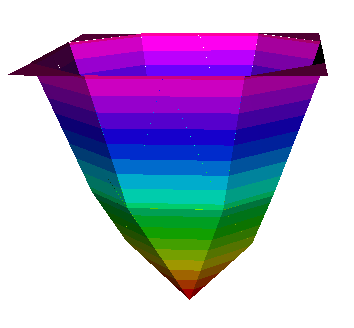
\includegraphics[scale=0.16]{img/Difusion/Recortes/steady_diffusion_exact_n_4.png}
				\caption{Solución exacta.}
			\end{subfigure}
			\begin{subfigure}[b]{0.215\textwidth}
				\centering
				
\includegraphics[scale=0.16]{img/Difusion/Recortes/steady_diffusion_approx_n_4.png}
				\caption{Solución discreta.}
			\end{subfigure}
			\begin{subfigure}[b]{0.11\textwidth}
				\centering
				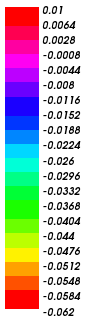
\includegraphics[scale=0.23]{img/Difusion/Recortes/steady_diffusion_values.png}
				%\caption*{ }
			\end{subfigure}
			\begin{subfigure}[b]{0.215\textwidth}
				\centering
				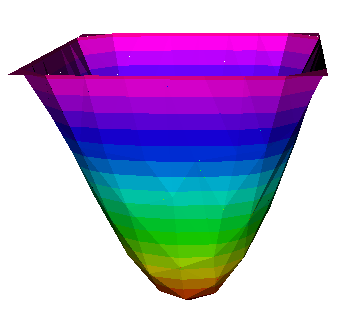
\includegraphics[scale=0.16]{img/Difusion/Recortes/steady_diffusion_exact_n_8.png}
				\caption{Solución exacta.}
			\end{subfigure}
			\begin{subfigure}[b]{0.215\textwidth}
				\centering
				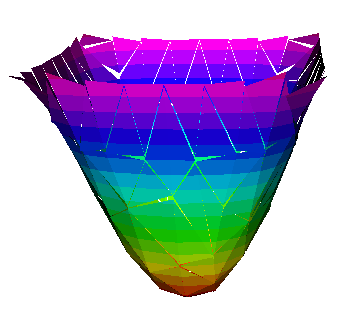
\includegraphics[scale=0.16]{img/Difusion/Recortes/steady_diffusion_approx_n_8.png}
				\caption{Solución discreta.}
			\end{subfigure}
			\caption{A la izquierda $h\approx\frac{1}{4}$. A la derecha $h\approx\frac{1}{8}$}
		\end{figure}
		\begin{figure}[h!]
			\begin{subfigure}[b]{0.215\textwidth}
				\centering
				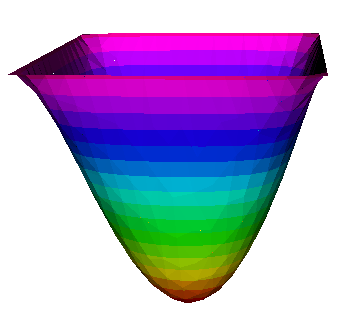
\includegraphics[scale=0.16]{img/Difusion/Recortes/steady_diffusion_exact_n_16.png}
				\caption{Solución exacta.}
			\end{subfigure}
			\begin{subfigure}[b]{0.215\textwidth}
				\centering
				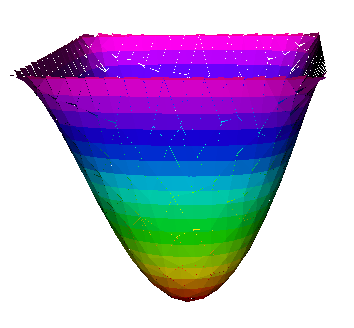
\includegraphics[scale=0.16]{img/Difusion/Recortes/steady_diffusion_approx_n_16.png}
				\caption{Solución discreta.}
			\end{subfigure}
			\begin{subfigure}[b]{0.11\textwidth}
				\centering
				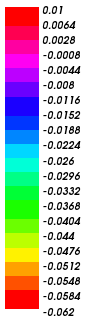
\includegraphics[scale=0.23]{img/Difusion/Recortes/steady_diffusion_values.png}
				%\caption*{ }
			\end{subfigure}
			\begin{subfigure}[b]{0.215\textwidth}
				\centering
				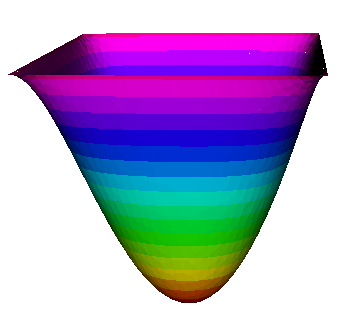
\includegraphics[scale=0.16]{img/Difusion/Recortes/steady_diffusion_exact_n_32.png}
				\caption{Solución exacta.}
			\end{subfigure}
			\begin{subfigure}[b]{0.215\textwidth}
				\centering
				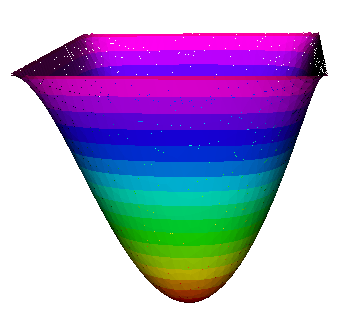
\includegraphics[scale=0.16]{img/Difusion/Recortes/steady_diffusion_approx_n_32.png}
				\caption{Solución discreta.}
			\end{subfigure}
			\caption{A la izquierda $h\approx\frac{1}{16}$. A la derecha $h\approx\frac{1}{32}$}
		\end{figure}
		\end{frame}
		
		\begin{frame}{Errores con $\sigma=4$ y $\mathbb{P}^2_1(\T_h)$}
		\begin{minipage}{0.50\textwidth}
			\centering
			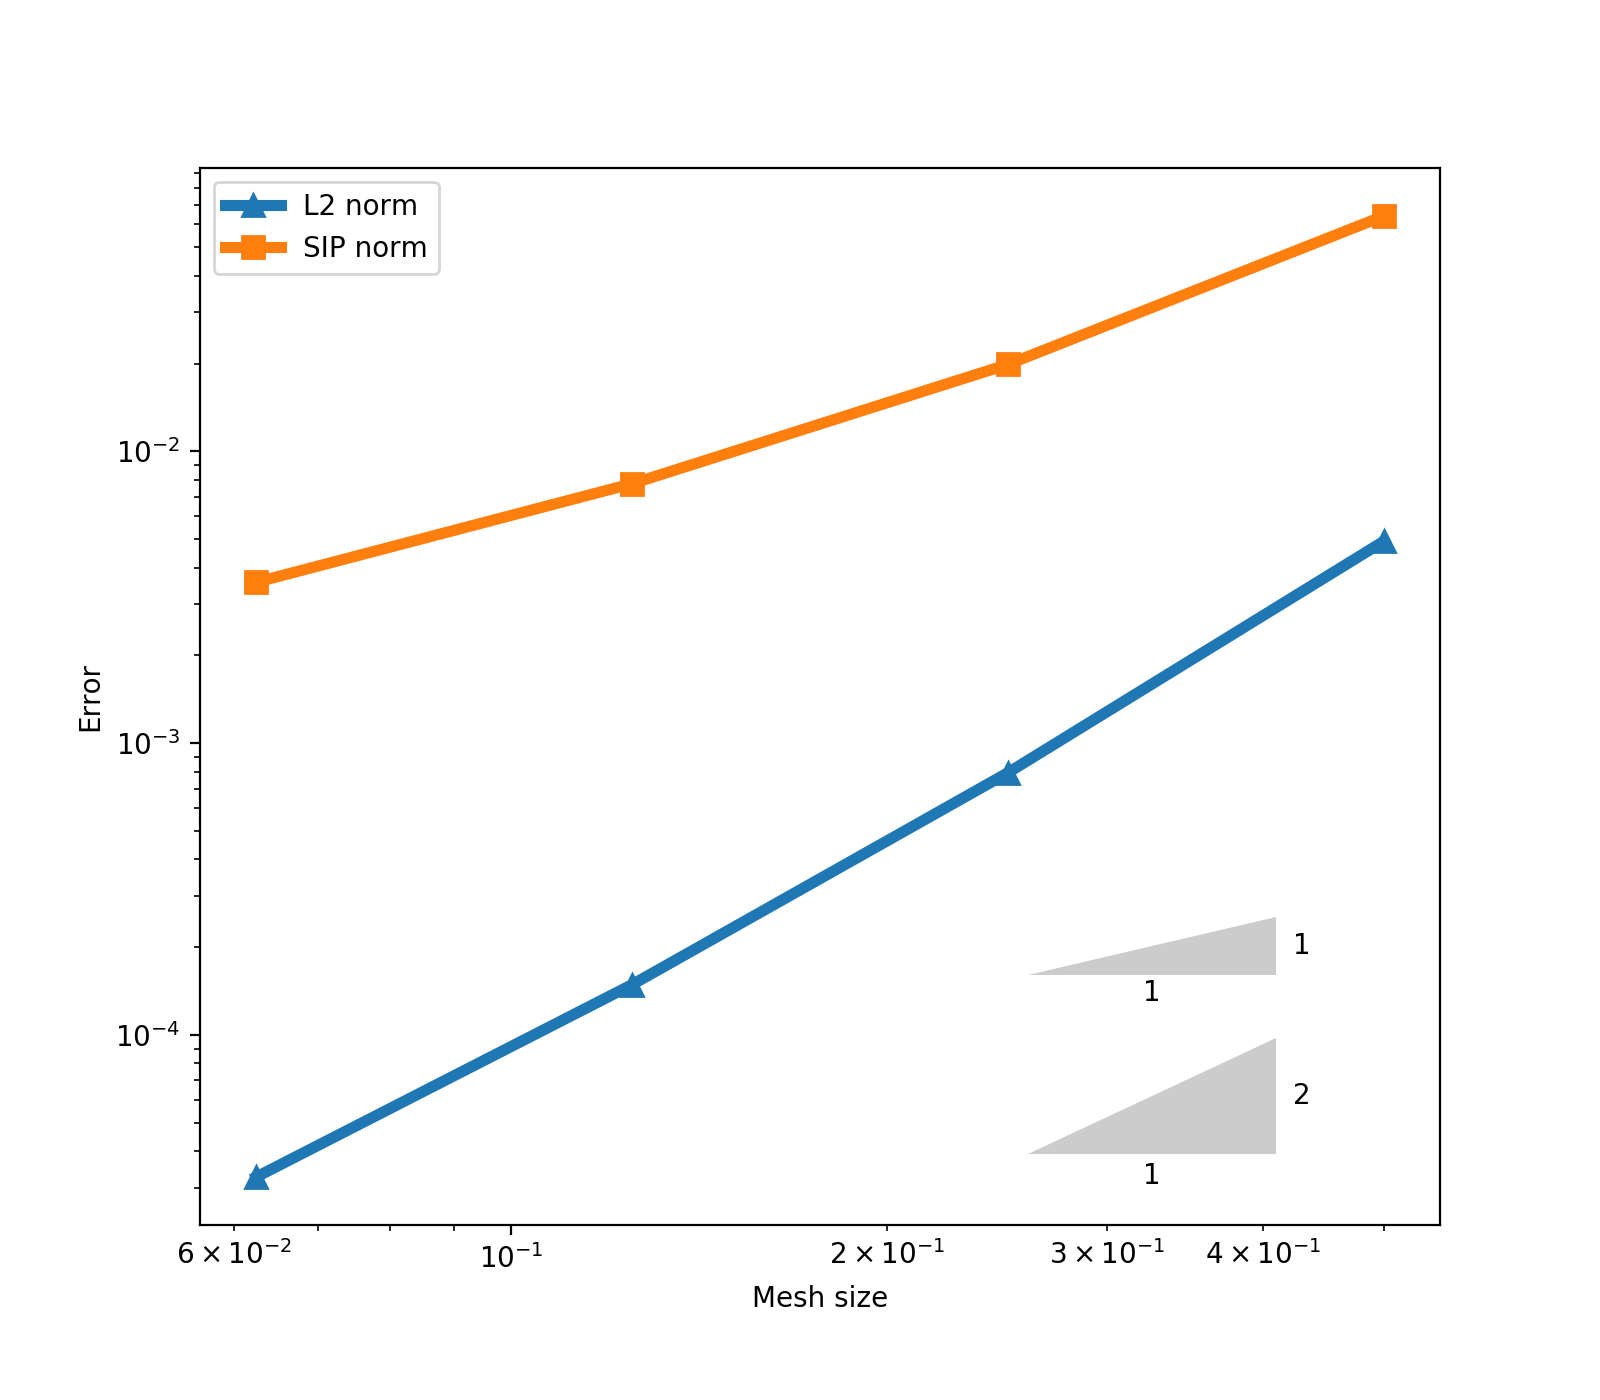
\includegraphics[scale=0.30]{img/Difusion/errores_difusion_P1dc.png}
			\captionof{figure}{Errores en escala logarítmica.}
		\end{minipage}
		\begin{minipage}{0.49\textwidth}
			\centering
			\begin{tabular}{|c|c|c|}
				\hline 
				\multirow{2}{*}{$h$} & \multicolumn{2}{c|}{Orden} \\
				\cline{2-3}
				&  $\normasip{\cdot}$ & $\norma{\cdot}_{L^2(\Omega)}$ \\ 
				\hline
				\hline
				$\frac{1}{4}\to\frac{1}{8}$ & $1.69$ & $2.6$ \\ 
				\hline 
				$\frac{1}{8}\to\frac{1}{16}$ & $1.36$ & $2.41$ \\ 
				\hline 
				$\frac{1}{16}\to\frac{1}{32}$ & $1.12$ & $2.19$\\
				\hline
			\end{tabular}
			\captionof{table}{Orden de convergencia.}
		\end{minipage}
		\end{frame}
		
		
		\begin{frame}{Errores con $\sigma=10$ y $\mathbb{P}^2_2(\T_h)$}
		\begin{minipage}{0.49\textwidth}
			\centering
			\begin{tabular}{|c|c|c|}
				\hline 
				\multirow{2}{*}{$h$} & \multicolumn{2}{c|}{Orden} \\
				\cline{2-3}
				&  $\normasip{\cdot}$ & $\norma{\cdot}_{L^2(\Omega)}$ \\ 
				\hline
				\hline
				$\frac{1}{4}\to\frac{1}{8}$ & $2.24$ & $3.16$ \\ 
				\hline 
				$\frac{1}{8}\to\frac{1}{16}$ & $2.1$ & $3.06$ \\ 
				\hline 
				$\frac{1}{16}\to\frac{1}{32}$ & $1.95$ & $2.95$\\
				\hline
			\end{tabular}
			\captionof{table}{Orden de convergencia.}
		\end{minipage}
		\begin{minipage}{0.5\textwidth}
			\centering
			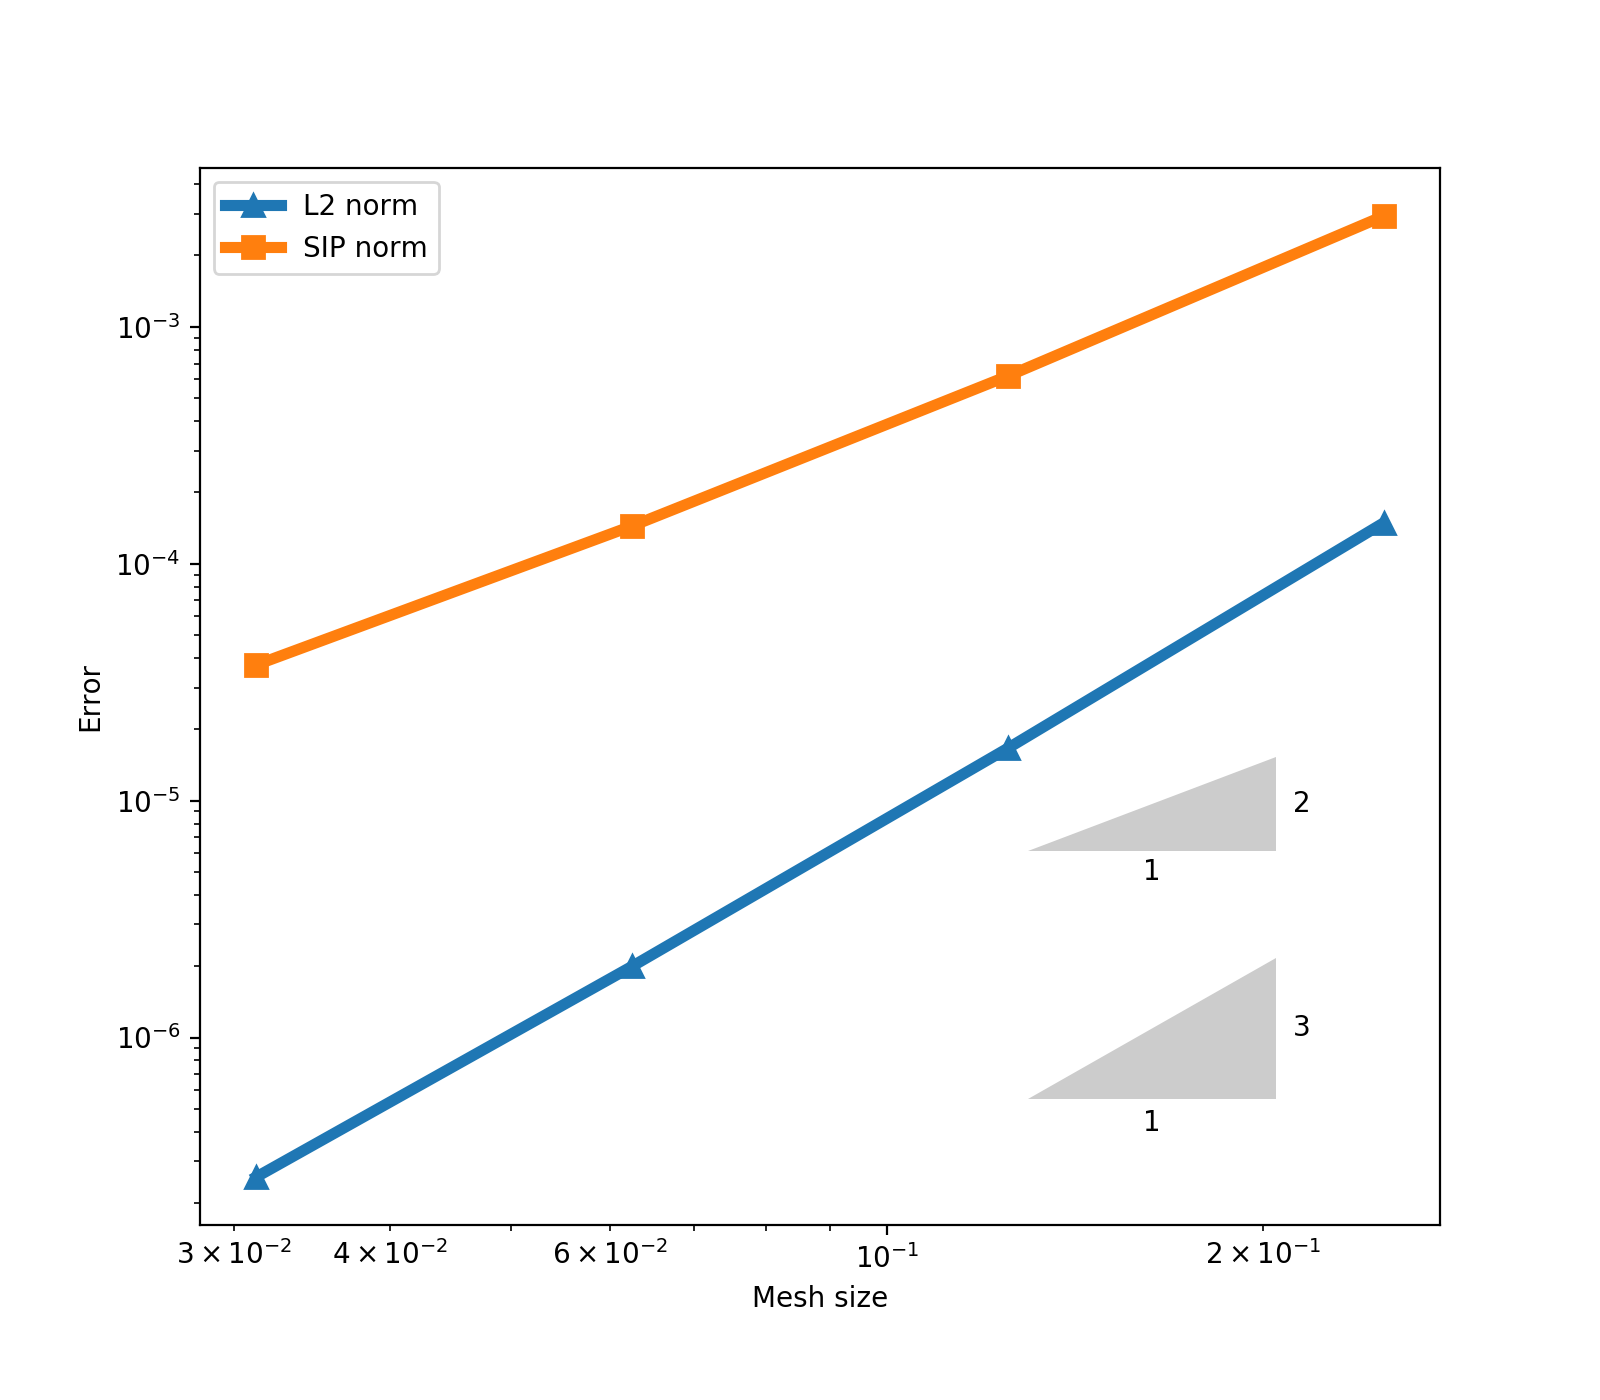
\includegraphics[scale=0.30]{img/Difusion/errores_difusion_P2dc.png}
			\captionof{figure}{Errores en escala logarítmica.}
		\end{minipage}
		\end{frame}
		
		\begin{frame}{Soluciones al variar $\sigma$ con $\mathbb{P}_1^2(\T_h)$}
		
		\begin{figure}[h!]
			\begin{subfigure}[b]{0.27\textwidth}
				\centering
				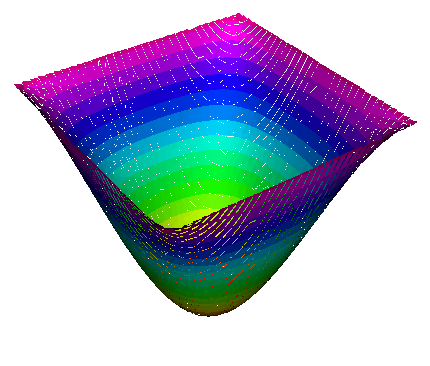
\includegraphics[scale=0.20]{img/Difusion/Recortes/steady_diffusion_approx_sigma_0_01.png}
				\caption{$\sigma=0,01$.}
			\end{subfigure}
			\begin{subfigure}[b]{0.27\textwidth}
				\centering
				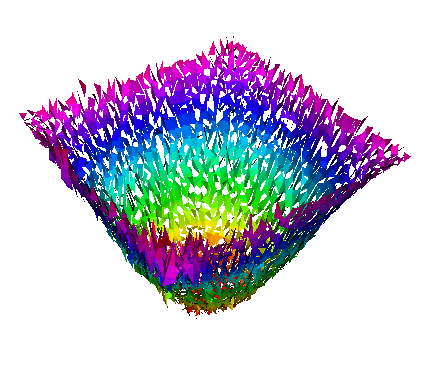
\includegraphics[scale=0.20]{img/Difusion/Recortes/steady_diffusion_approx_sigma_0_5.png}
				\caption{$\sigma=0,5$.}
			\end{subfigure}
			\begin{subfigure}[b]{0.27\textwidth}
				\centering
				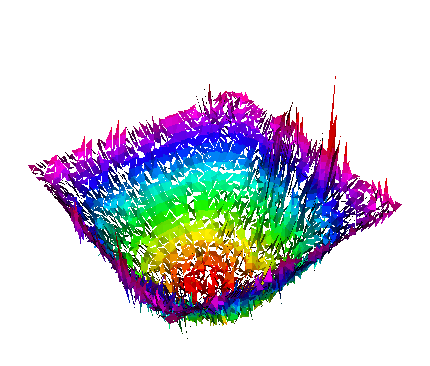
\includegraphics[scale=0.20]{img/Difusion/Recortes/steady_diffusion_approx_sigma_1.png}
				\caption{$\sigma=1$.}
			\end{subfigure}
			\begin{subfigure}[b]{0.15\textwidth}
				\centering
				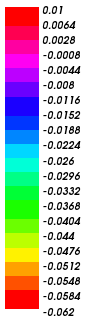
\includegraphics[scale=0.25]{img/Difusion/Recortes/steady_diffusion_values.png}
				%\caption*{ }
			\end{subfigure}
			%\end{figure}
			%\begin{figure}
			%	\ContinuedFloat
			\begin{subfigure}[b]{0.27\textwidth}
				\centering
				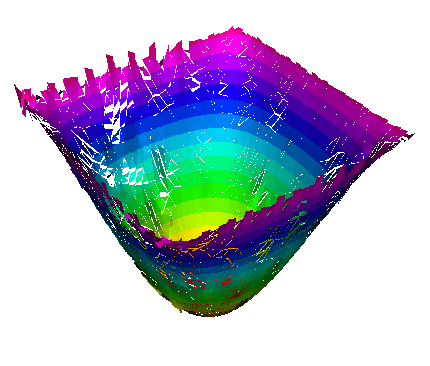
\includegraphics[scale=0.20]{img/Difusion/Recortes/steady_diffusion_approx_sigma_2.png}
				\caption{$\sigma=2$.}
			\end{subfigure}
			\begin{subfigure}[b]{0.27\textwidth}
				\centering
				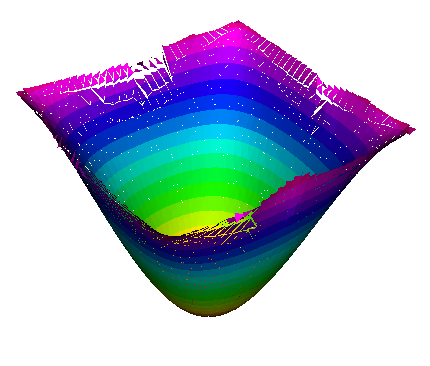
\includegraphics[scale=0.20]{img/Difusion/Recortes/steady_diffusion_approx_sigma_3.png}
				\caption{$\sigma=3$.}
			\end{subfigure}
			\begin{subfigure}[b]{0.27\textwidth}
				\centering
				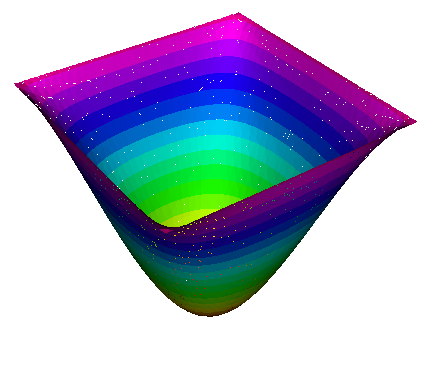
\includegraphics[scale=0.20]{img/Difusion/Recortes/steady_diffusion_approx_sigma_4.png}
				\caption{$\sigma=4$.}
			\end{subfigure}
			\begin{subfigure}[b]{0.15\textwidth}
				\centering
				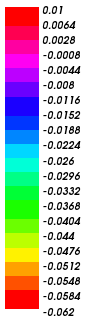
\includegraphics[scale=0.25]{img/Difusion/Recortes/steady_diffusion_values.png}
				%\caption*{ }
			\end{subfigure}
			\caption{Gráficas de soluciones discretas con $h\approx\frac{1}{32}$.}
		\end{figure}
		
		\end{frame}
		
		\begin{frame}{Errores al variar $\sigma$ con $\mathbb{P}_1^2(\T_h)$}
			\begin{figure}[h!]
				\centering
				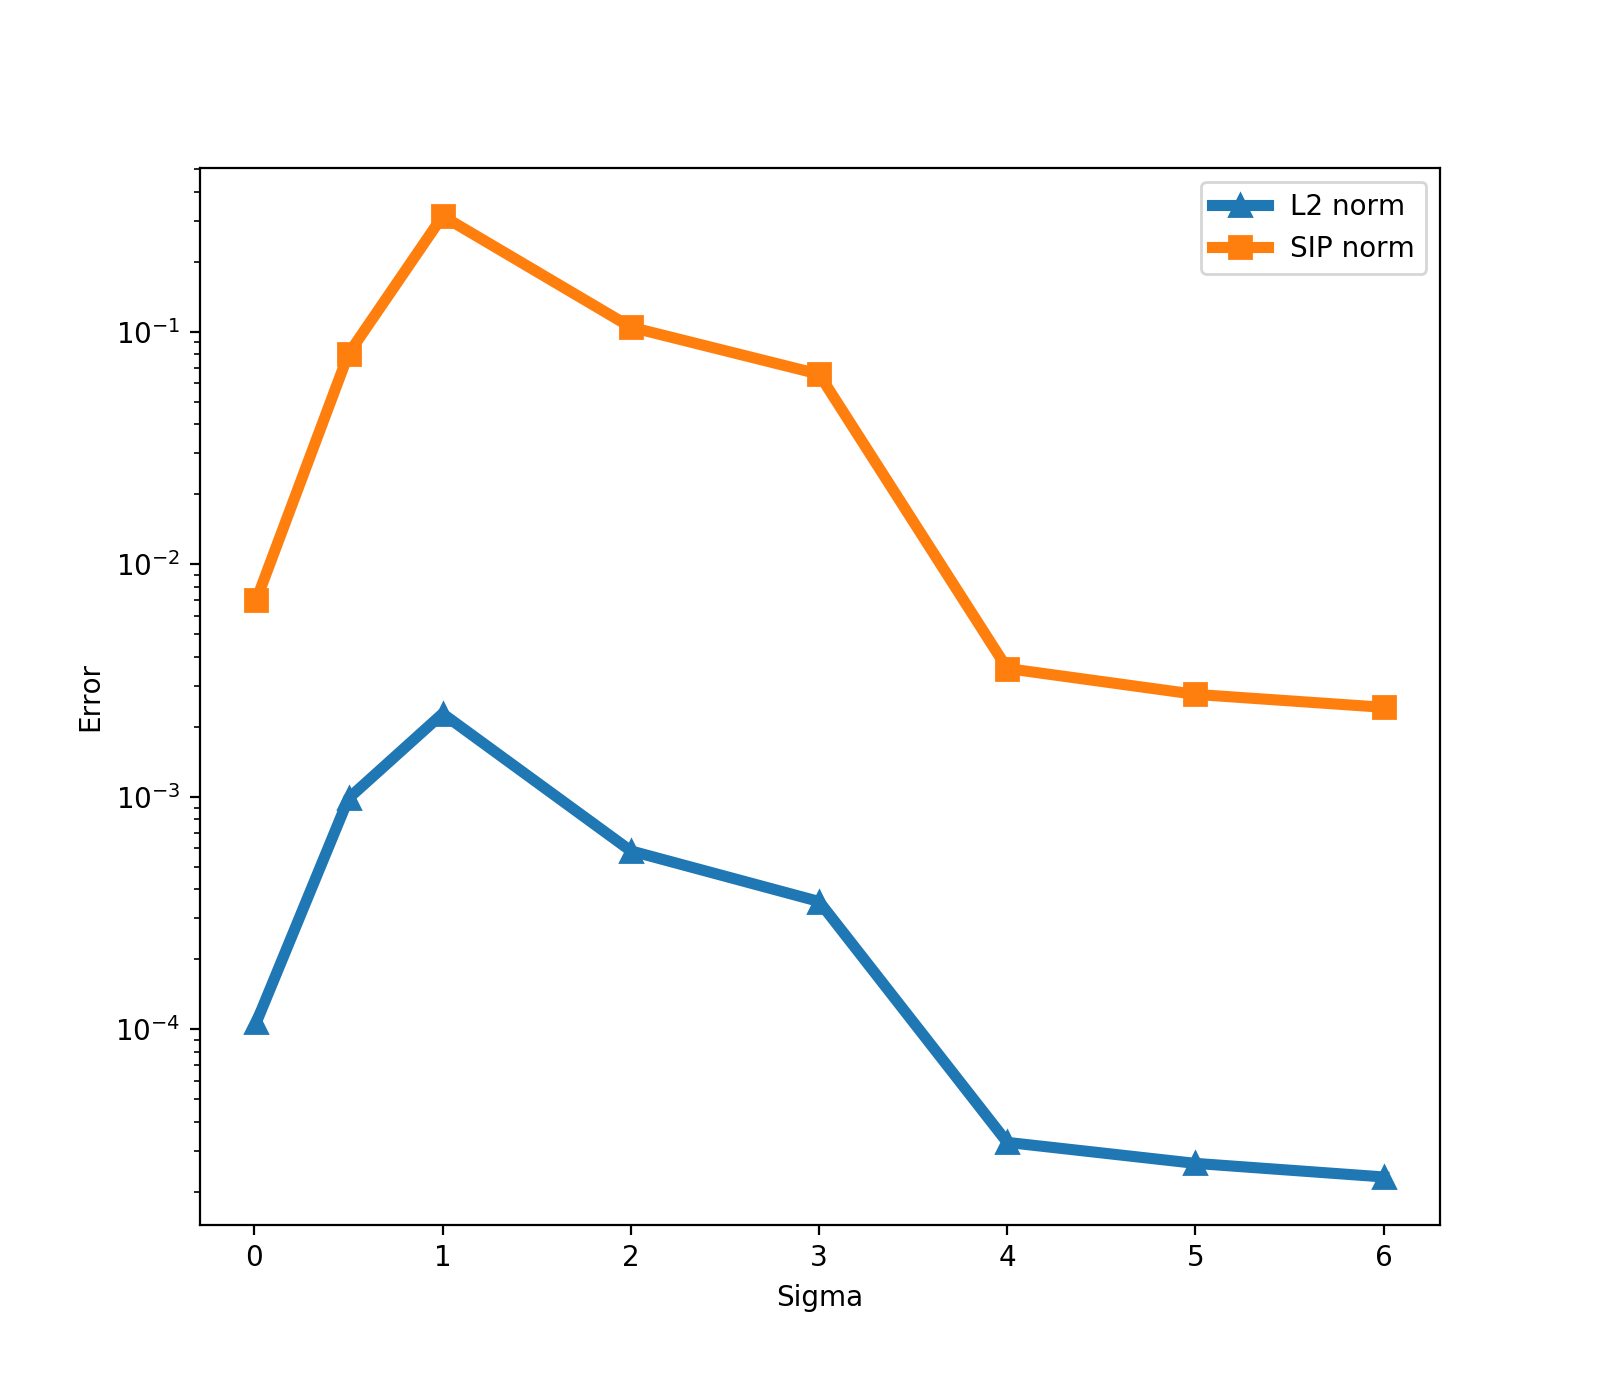
\includegraphics[scale=0.37]{img/Difusion/errores_difusion_sigma.png}
				\caption{Errores con $h\approx\frac{1}{32}$.}
			\end{figure}
		\end{frame}

	\subsection{Hyperbollic problem}
	
	\begin{frame}{Problema modelo}
		Consideramos el problema de convección-reacción:
		\begin{block}{}
		\begin{equation*}
		\label{prob_modelo_hiperbolica}
		\left\{
		\begin{aligned}
		\beta\cdot\nabla u+\mu u&=f & \text{en } &\Omega, \\
		u&=0 & \text{en } &\partial\Omega^-,
		\end{aligned}
		\right.
		\end{equation*}
		\end{block}
		donde 
		\begin{itemize}
			\item $\partial\Omega^-=\left\{x\in\partial\Omega\colon \beta(x)\mathbf{n}(x)<0\right\},$
			\item $\mu\in L^\infty(\Omega)$,
			\item $\beta\in\left[\text{Lip}(\Omega)\right]^d$,
			\item $f\in L^2(\Omega)$.
		\end{itemize}
		\vspace*{.5cm}
		Asumimos que existe $\mu_0>0$ tal que $\displaystyle\mu-\frac{1}{2}\nabla\cdot\beta\geq\mu_0$ en $\Omega$.
		
	\end{frame}

	\subsubsection{Numerical approximation}
	
	\begin{frame}{Espacio finito-dimensional}
	
	\textbf{Espacio finito-dimensional}: $$V_h\coloneqq\alert{\mathbb{P}_k^d(\T_h)}$$ con base $\left\{\phi_i\right\}_{i=1}^{N_h^{\text{cf}}}$.
	\vspace*{1cm}
	
	Denotamos:
	\begin{itemize}
		\item $V_*\coloneqq V\cap H^1(\T_h)$;
		\item $V_{*h}\coloneqq V_*+V_h$.
	\end{itemize}
	\end{frame}
	
	\begin{frame}{Método de los Flujos Centrados}
	\begin{itemize}\itemsep1em
		\item $a_h^{\text{cf}}\colon V_{*h}\times V_h\to\R$,
		\begin{align*}
		\alert{\acf{u}{v_h}}&\coloneqq\framedmath<2>{\displaystyle \int_\Omega(\beta\cdot\nabla_h u)v_h+\int_\Omega\mu u v_h}\\&\framedmath<3>{\displaystyle +\int_{\partial\Omega}(\beta\mathbf{n})^-uv_h}\framedmath<4>{\displaystyle -\sum_{e\in\E_h^i}\int_e(\beta\cdot\mathbf{n}_e)\salto{u}\media{v_h}};
		\end{align*}
		\begin{itemize}
			\item<2> \myframed{Términos anteriores.}
			\item<3> \myframed{Condiciones de frontera de forma débil.}
			\item<4> \myframed{Coercitividad.}
		\end{itemize}
		\item $L_h\colon V_h\to\R$, $\displaystyle \alert{L_h(v_h)}\coloneqq\int_\Omega f v_h.$
	\end{itemize}
\end{frame}

\begin{frame}{Problema discreto}
	\begin{itemize}
		\item $\text{Encontrar }u_h\in V_h\text{ tal que }\acf{u_h}{v_h}=L_h(v_h)\text{ para todo }v_h\in V_h$.
	\end{itemize}
	\vspace*{0.1cm}
	$$\Big{\Updownarrow}$$
	\vspace*{-0.3cm}
	\begin{itemize}
		\item Resolver el sistema lineal $A^{\text{cf}}\mathbf{U}^{\text{cf}}=\mathbf{F}^{\text{cf}}$ donde:
		\vspace*{0.3cm}
		\begin{itemize}
			\item $A^{\text{cf}}=\left(A_{ij}^{\text{cf}}\right)_{i,j\in\left\{1,2,\ldots,N_h^{\text{cf}}\right\}}$ con $A_{ij}^{\text{cf}}=\acf{\phi_j}{\phi_i}$;
			\item $\mathbf{U}^{\text{cf}}=\left(U_1^{\text{cf}},U_2^{\text{cf}},\ldots,U_{N_h^{\text{cf}}}^{\text{cf}}\right)^t$ con $u_h=\displaystyle\sum_{i=1}^{N_h^{\text{cf}}}U_i^{\text{cf}}\phi_i$;
			\item $\mathbf{F}^{\text{cf}}=\left(F_1^{\text{cf}},F_2^{\text{cf}},\ldots,F_{N_h^{\text{cf}}}^{\text{cf}}\right)^t$ con $F_i^{\text{cf}}=L_h(\phi_i)$.
		\end{itemize}
	\end{itemize}
	
	\vspace*{0.3cm}
	El problema discreto es consistente con el problema modelo en $V_*$.
	
	\end{frame}
	
	\begin{frame}[allowframebreaks]{Propiedades del problema discreto}
	\begin{definicion}
		En el espacio $V_{*h}$ se define la norma $\normacf{\cdot}\colon V_{*h}\to\R$ como $$\normacf{u}\coloneqq\escalarcf{u}{u}^{1/2}= \left(\max\{\norma{\mu}_{L^\infty(\Omega)},C_\beta\}\norma{u}_{L^2(\Omega)}^2+\frac{1}{2}\norma{u}_{L^2(|\beta\cdot\mathbf{n}|;\partial\Omega)}^2\right)^{1/2}.$$
	\end{definicion}
	\framebreak
	\begin{lemma}
		La forma bilineal $\acf{\cdot}{\cdot}$ es continua en $V_h$ con la norma $\normacf{\cdot}$, esto es, existe $C>0$ tal que para todos $u_h,v_h\in V_h$ se verifica que $$\acf{u_h}{v_h}\leq C\normacf{u_h}\normacf{v_h}.$$
	\end{lemma}
	
	\begin{lemma}
		La forma bilineal $\acf{\cdot}{\cdot}$ es coercitiva en $V_h$ con la norma $\normacf{\cdot}$, esto es, existe $C>0$ tal que para todo $v_h\in V_h$ se verifica que $$\acf{v_h}{v_h}\geq C\normacf{v_h}^2.$$
	\end{lemma}
	\framebreak
	\begin{lemma}
		El problema de encontrar $u_h\in V_h$ tal que $$\acf{u_h}{v_h}=L_h(v_h)$$ para todo $v_h\in V_h$ tiene solución y es única.
	\end{lemma}
	\textbf{Demostraciones}:
	\begin{enumerate}
		\item Lax-Milgram.
		\item Unicidad de solución.
	\end{enumerate}
	
	\end{frame}
	
	\begin{frame}{Análisis de errores}
	\begin{theorem}
		\label{theorem:hiperbolico_CF_orden_norma_CF}
		Sea $u\in H^{k+1}(\Omega)$, $k\in\N$ la solución del problema modelo y sea $u_h\in \mathbb{P}_k^d(\T_h)$ la solución del problema discreto.
		
		Entonces existe $C>0$ independiente de $h$ y dependiente de los datos únicamente a través del factor $\left(\min\{1,\max\{\norma{\mu}_{L^\infty(\Omega)},C_\beta\}\mu_0\}\right)^{-1}$ tal que
		\begin{equation*}
		\label{theorem:orden_convergencia_CF}
		\normacf{u-u_h}\leq C\norma{u}_{H^{k+1}(\Omega)}h^k.
		\end{equation*}
	\end{theorem}
	\end{frame}
	
	\begin{frame}{Método de Aguas Arriba}
	
	\begin{itemize}\itemsep1em
		\item $a_h^{\text{upw}}\colon V_{*h}\times V_h\to \R$, $$\alert{\aupw{u}{v_h}}\coloneqq \framedmath<2>{\displaystyle \acf{u}{v_h}}+\framedmath<3>{\displaystyle \sum_{e\in\E_h^i}\int_e\frac{\eta}{2}|\beta\cdot\mathbf{n}_e|\salto{u}\salto{v_h}};$$
		\begin{itemize}
			\item<2> \myframed{Método de los Flujos Centrados.}
			\item<3> \myframed{Estabilidad.}
		\end{itemize}
		\item $L_h\colon V_h\to\R$, $\displaystyle \alert{L_h(v_h)}\coloneqq\int_\Omega f v_h.$
	\end{itemize}
	\end{frame}
	
	\begin{frame}{Problema discreto}
	
	\begin{itemize}
		\item $\text{Encontrar }u_h\in V_h\text{ tal que }\aupw{u_h}{v_h}=L_h(v_h)\text{ para todo }v_h\in V_h$.
	\end{itemize}
	\vspace*{0.1cm}
	$$\Big{\Updownarrow}$$
	\vspace*{-0.3cm}
	\begin{itemize}
		\item Resolver el sistema lineal $A^{\text{upw}}\mathbf{U}^{\text{upw}}=\mathbf{F}^{\text{upw}}$ donde:
		\vspace*{0.3cm}
		\begin{itemize}
			\item $A^{\text{upw}}=\left(A_{ij}^{\text{upw}}\right)_{i,j\in\left\{1,2,\ldots,N_h^{\text{upw}}\right\}}$ con $A_{ij}^{\text{upw}}=\aupw{\phi_j}{\phi_i}$;
			\item $\mathbf{U}^{\text{upw}}=\left(U_1^{\text{upw}},U_2^{\text{upw}},\ldots,U_{N_h^{\text{upw}}}^{\text{upw}}\right)^t$ con $u_h=\displaystyle\sum_{i=1}^{N_h^{\text{upw}}}U_i^{\text{upw}}\phi_i$;
			\item $\mathbf{F}^{\text{upw}}=\left(F_1^{\text{upw}},F_2^{\text{upw}},\ldots,F_{N_h^{\text{upw}}}^{\text{upw}}\right)^t$ con $F_i^{\text{upw}}=L_h(\phi_i)$.
		\end{itemize}
	\end{itemize}
	
	\vspace*{0.3cm}
	El problema discreto es consistente con el problema modelo en $V_*$.
	
	\end{frame}
	
	\begin{frame}[allowframebreaks]{Propiedades del problema discreto}
	\begin{definicion}
		En el espacio $V_{*h}$ se define la norma $\normaupw{\cdot}\colon V_{*h}\to\R$ como $$\normaupw{u}\coloneqq\escalarupw{u}{u}^{1/2}= \left(\normacf{u}^2+\frac{\eta}{2}\sum_{e\in\E_h^i}\norma{\salto{u}}^2_{L^2(|\beta\cdot\mathbf{n}_e|;e)} \right)^{1/2}.$$
	\end{definicion}
	\framebreak
	\begin{lemma}
		La forma bilineal $\aupw{\cdot}{\cdot}$ es continua en $V_h$ con la norma $\normaupw{\cdot}$, esto es, existe $C>0$ tal que para todos $u_h,v_h\in V_h$ se verifica que $$\aupw{u_h}{v_h}\leq C\normaupw{u_h}\normaupw{v_h}.$$
	\end{lemma}
	
	\begin{proposition}
		La forma bilineal $\aupw{\cdot}{\cdot}$ es coercitiva en $V_h$ con la norma $\normaupw{\cdot}$, esto es, existe $C>0$ tal que para todo $v_h\in V_h$ se verifica que $$\aupw{v_h}{v_h}\geq C\normaupw{v_h}^2.$$
	\end{proposition}
	\framebreak
	\begin{lemma}
		El problema de encontrar $u_h\in V_h$ tal que $$\aupw{u_h}{v_h}=L_h(v_h)$$ para todo $v_h\in V_h$ tiene solución y es única.
	\end{lemma}
	\textbf{Demostraciones}:
	\begin{enumerate}
		\item Lax-Milgram.
		\item Unicidad de solución.
	\end{enumerate}
	\end{frame}
	
	\begin{frame}{Análisis de errores}
	\begin{theorem}
		\label{theorem:hiperbolico_UPW_orden_norma_UPW}
		Sea $u\in H^{k+1}(\Omega)$, $k\in\N$ la solución del problema modelo y sea $u_h\in \mathbb{P}_k^d(\T_h)$ la solución del problema discreto.
		
		Entonces existe $C>0$ independiente de $h$ y dependiente de los datos únicamente a través del factor $\left(\min\{1,\max\{\norma{\mu}_{L^\infty(\Omega)},C_\beta\}\mu_0\}\right)^{-1}$ tal que $$\normaupw{u-u_h}\leq C\norma{u}_{H^{k+1}(\Omega)}h^{k+1/2}.$$
	\end{theorem}
\end{frame}

	\subsubsection{Numerical experiments}
	\begin{frame}{Problema hiperbólico}
		Consideramos el problema hiperbólico:
		\begin{block}{}
		\begin{equation*}
		\left\{
		\begin{aligned}
		\beta\cdot\nabla u+\mu u&=f & \text{en } &\Omega, \\
		u&=0 & \text{en } &\partial\Omega^-,
		\end{aligned}
		\right.
		\end{equation*}
		\end{block}
		con
		\begin{itemize}
			\item $d=2$;
			\item $\Omega=\left\{(x,y)\in\R^2\colon x^2+y^2<1 \right\}$;
			\item $A=10$, $x_0=y_0=0.3$;
			\item $\mu=2A$;
			\item $\beta(x,y)\coloneqq(y,-x)$;
			\item $f\colon\Omega\to\R$, $f(x,y)\coloneqq \mu e^{-A\left((x-x_0)^2+(y-y_0)^2\right)}(x_0 y -x y_0 + 1)$.
		\end{itemize}
		
		\vspace*{0.3cm}
		$u_{\text{ex}}\colon\Omega\to\R$ definida como
		\begin{equation*}
		\label{sol_experimento_hiperbolico}
		\uex (x,y)\coloneqq e^{-A\left((x-x_0)^2+(y-y_0)^2\right)}
		\end{equation*}
		es la \alert{única solución exacta} ($\alert{u_\text{ex}\in V}$).
		
		\end{frame}
		
		\begin{frame}{Soluciones con $\mathbb{P}_1^2(\T_h)$}
		\vspace{-0.2cm}
		\begin{figure}[h!]
			\begin{subfigure}[b]{0.27\textwidth}
				\centering
				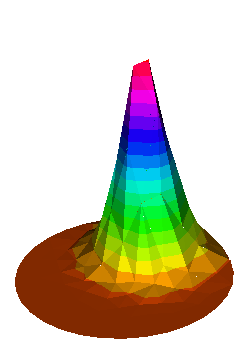
\includegraphics[scale=0.22]{img/Conveccion_Reaccion/Recortes/steady_convect_react_exact_n_32.png}
				\caption{Solución exacta.}
			\end{subfigure}
			\begin{subfigure}[b]{0.27\textwidth}
				\centering
				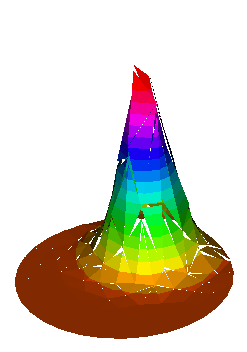
\includegraphics[scale=0.22]{img/Conveccion_Reaccion/Recortes/steady_convect_react_approx_CF_n_32.png}
				\caption{Flujos Centrados.}
			\end{subfigure}
			\begin{subfigure}[b]{0.27\textwidth}
				\centering
				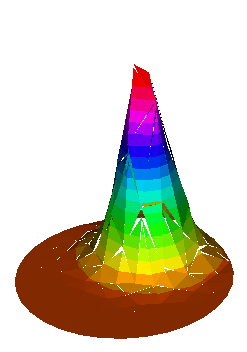
\includegraphics[scale=0.22]{img/Conveccion_Reaccion/Recortes/steady_convect_react_approx_UPW_n_32.png}
				\caption{Aguas Arriba.}
			\end{subfigure}
			\begin{subfigure}[b]{0.15\textwidth}
				\centering
				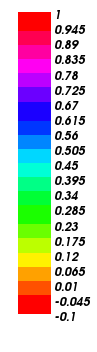
\includegraphics[scale=0.22]{img/Conveccion_Reaccion/Recortes/steady_convect_react_values.png}
				%\caption*{ }
			\end{subfigure}
			\caption{Gráficas obtenidas con $h\approx\frac{\pi}{16}$.}
		\end{figure}
		\vspace{-0.7cm}
		\begin{figure}[h!]
			\begin{subfigure}[b]{0.27\textwidth}
				\centering
				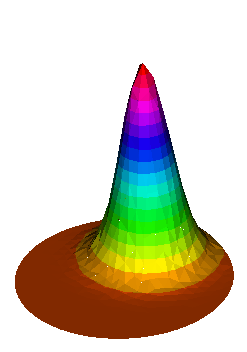
\includegraphics[scale=0.22]{img/Conveccion_Reaccion/Recortes/steady_convect_react_exact_n_64.png}
				\caption{Solución exacta.}
			\end{subfigure}
			\begin{subfigure}[b]{0.27\textwidth}
				\centering
				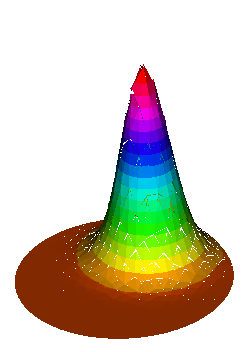
\includegraphics[scale=0.22]{img/Conveccion_Reaccion/Recortes/steady_convect_react_approx_CF_n_64.png}
				\caption{Flujos Centrados.}
			\end{subfigure}
			\begin{subfigure}[b]{0.27\textwidth}
				\centering
				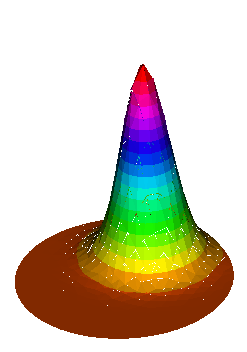
\includegraphics[scale=0.22]{img/Conveccion_Reaccion/Recortes/steady_convect_react_approx_UPW_n_64.png}
				\caption{Aguas Arriba.}
			\end{subfigure}
			\begin{subfigure}[b]{0.15\textwidth}
				\centering
				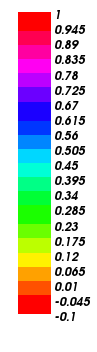
\includegraphics[scale=0.22]{img/Conveccion_Reaccion/Recortes/steady_convect_react_values.png}
				%\caption*{ }
			\end{subfigure}
			\caption{Gráficas obtenidas con $h\approx\frac{\pi}{32}$.}
		\end{figure}
		\end{frame}
		
		\begin{frame}{Soluciones con $\mathbb{P}_1^2(\T_h)$}
		\vspace{-0.2cm}
		\begin{figure}[h!]
			\begin{subfigure}[b]{0.27\textwidth}
				\centering
				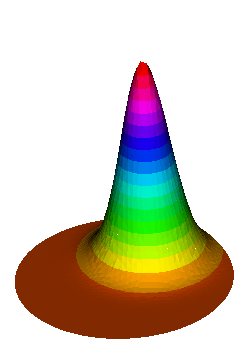
\includegraphics[scale=0.22]{img/Conveccion_Reaccion/Recortes/steady_convect_react_exact_n_128.png}
				\caption{Solución exacta.}
			\end{subfigure}
			\begin{subfigure}[b]{0.27\textwidth}
				\centering
				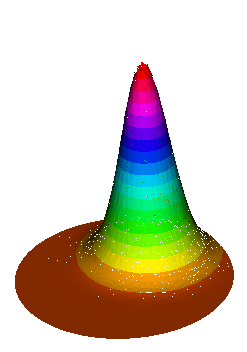
\includegraphics[scale=0.22]{img/Conveccion_Reaccion/Recortes/steady_convect_react_approx_CF_n_128.png}
				\caption{Flujos Centrados.}
			\end{subfigure}
			\begin{subfigure}[b]{0.27\textwidth}
				\centering
				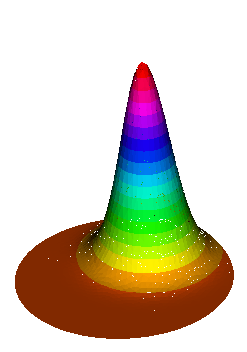
\includegraphics[scale=0.22]{img/Conveccion_Reaccion/Recortes/steady_convect_react_approx_UPW_n_128.png}
				\caption{Aguas Arriba.}
			\end{subfigure}
			\begin{subfigure}[b]{0.15\textwidth}
				\centering
				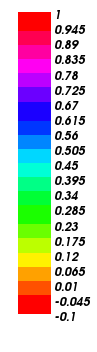
\includegraphics[scale=0.22]{img/Conveccion_Reaccion/Recortes/steady_convect_react_values.png}
				%\caption*{ }
			\end{subfigure}
			\caption{Gráficas obtenidas con $h\approx\frac{\pi}{64}$.}
		\end{figure}
		\vspace{-0.7cm}
		\begin{figure}[h!]
			\begin{subfigure}[b]{0.27\textwidth}
				\centering
				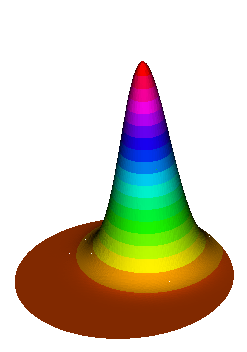
\includegraphics[scale=0.22]{img/Conveccion_Reaccion/Recortes/steady_convect_react_exact_n_256.png}
				\caption{Solución exacta.}
			\end{subfigure}
			\begin{subfigure}[b]{0.27\textwidth}
				\centering
				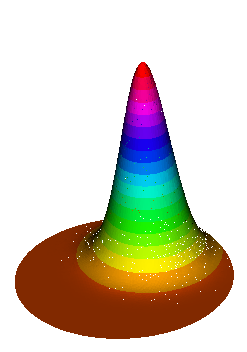
\includegraphics[scale=0.22]{img/Conveccion_Reaccion/Recortes/steady_convect_react_approx_CF_n_256.png}
				\caption{Flujos Centrados.}
			\end{subfigure}
			\begin{subfigure}[b]{0.27\textwidth}
				\centering
				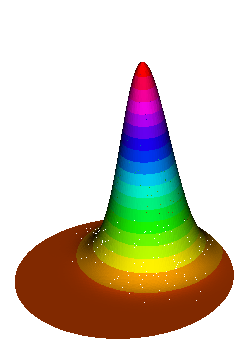
\includegraphics[scale=0.22]{img/Conveccion_Reaccion/Recortes/steady_convect_react_approx_UPW_n_256.png}
				\caption{Aguas Arriba.}
			\end{subfigure}
			\begin{subfigure}[b]{0.15\textwidth}
				\centering
				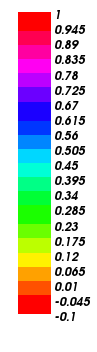
\includegraphics[scale=0.22]{img/Conveccion_Reaccion/Recortes/steady_convect_react_values.png}
				%\caption*{ }
			\end{subfigure}
			\caption{Gráficas obtenidas con $h\approx\frac{\pi}{128}$.}
		\end{figure}
		\end{frame}
		
		\begin{frame}{Errores con $\mathbb{P}_1^2(\T_h)$}
		\hspace{-0.3cm}
		\begin{minipage}{0.5\textwidth}
			\centering
			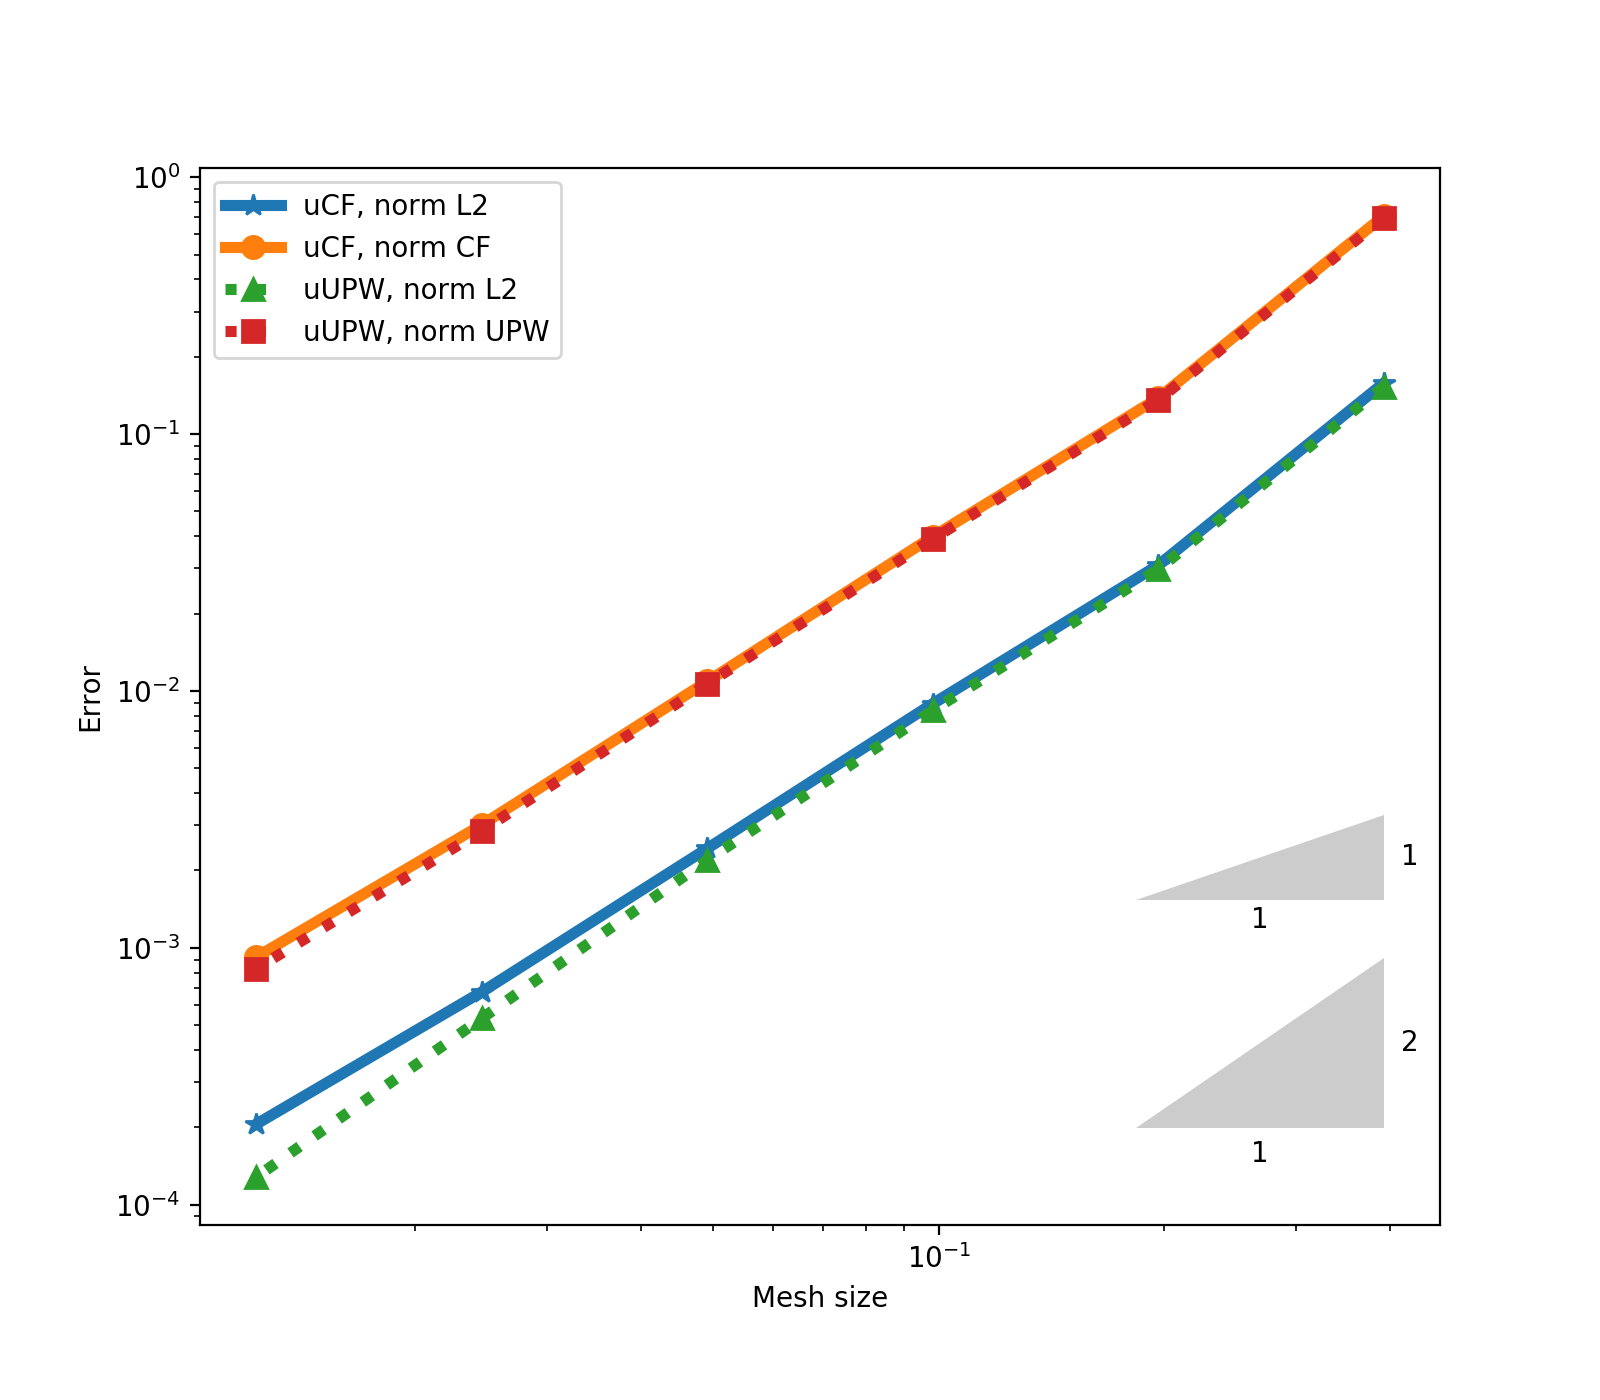
\includegraphics[scale=0.30]{img/Conveccion_Reaccion/errores_conveccion_reaccion_P1dc.png}
			\captionof{figure}{Errores en escala logarítmica.}
		\end{minipage}
		\begin{minipage}{0.49\textwidth}
			\small
			\centering
				\begin{tabular}{|c|c|c|c|}
					\hline
					\multirow{2}{*}{$h$} & \multicolumn{2}{c|}{Orden} & \multirow{2}{*}{Método}\\
					\cline{2-3}
					& $\norma{\cdot}_*$ & $\norma{\cdot}_{L^2(\Omega)}$ & \\ 
					\hline
					\hline
					\multirow{2}{*}{$\frac{\pi}{8}\to\frac{\pi}{16}$} & $2.36$ & $2.36$ & CF\\
					\cdashline{2-4}
					& $2.36$ & $2.36$ & UPW\\ 
					\hline 
					\multirow{2}{*}{$\frac{\pi}{16}\to\frac{\pi}{32}$} & $1.79$ & $1.79$ & CF\\
					\cdashline{2-4}
					
					& $1.79$ & $1.82$ & UPW\\
					\hline 
					\multirow{2}{*}{$\frac{\pi}{32}\to\frac{\pi}{64}$} & $1.87$ & $1.87$ & CF\\
					\cdashline{2-4}
					
					& $1.87$ & $1.94$ & UPW\\
					\hline
					\multirow{2}{*}{$\frac{\pi}{64}\to\frac{\pi}{128}$} & $1.85$ & $1.85$ & CF\\
					\cdashline{2-4}
					
					& $1.9$ & $2.04$ & UPW\\
					\hline
					\multirow{2}{*}{$\frac{\pi}{128}\to\frac{\pi}{256}$} & $1.71$ & $1.71$ & CF\\
					\cdashline{2-4}
					
					& $1.78$ & $2.05$& UPW\\
					\hline
				\end{tabular}
			%\captionof{table}{Orden de convergencia en cada iteración para ambos métodos en normas $\normacf{\cdot}$ o $\normaupw{\cdot}$ y $\norma{\cdot}_{L^2(\Omega)}$ con espacio discreto $\mathbb{P}^2_1(\T_h)$.}
			\captionof{table}{Orden de convergencia.}
		\end{minipage}
		
		\end{frame}
		
		\begin{frame}{Errores con $\mathbb{P}_2^2(\T_h)$}
		\hspace*{-0.5cm}
		\begin{minipage}{0.49\textwidth}
			\small
			\centering
				\begin{tabular}{|c|c|c|c|}
					\hline
					\multirow{2}{*}{$h$} & \multicolumn{2}{c|}{Orden} & \multirow{2}{*}{Método}\\
					\cline{2-3}
					& $\norma{\cdot}_*$ & $\norma{\cdot}_{L^2(\Omega)}$ & \\ 
					\hline
					\hline
					\multirow{2}{*}{$\frac{\pi}{8}\to\frac{\pi}{16}$} & $2.72$ & $2.72$ & CF\\
					\cdashline{2-4}
					& $2.69$ & $2.73$ & UPW\\ 
					\hline 
					\multirow{2}{*}{$\frac{\pi}{16}\to\frac{\pi}{32}$} & $2.8$ & $2.8$ & CF\\
					\cdashline{2-4}
					
					& $2.73$ & $2.84$ & UPW\\
					\hline 
					\multirow{2}{*}{$\frac{\pi}{32}\to\frac{\pi}{64}$} & $2.87$ & $2.87$ & CF\\
					\cdashline{2-4}
					
					& $2.69$ & $2.89$ & UPW\\
					\hline
					\multirow{2}{*}{$\frac{\pi}{64}\to\frac{\pi}{128}$} & $2.92$ & $2.92$ & CF\\
					\cdashline{2-4}
					
					& $2.68$ & $2.93$ & UPW\\
					\hline
					\multirow{2}{*}{$\frac{\pi}{128}\to\frac{\pi}{256}$} & $3.03$ & $3.03$ & CF\\
					\cdashline{2-4}
					
					& $2.7$ & $3.06$& UPW\\
					\hline
				\end{tabular}
			%\captionof{table}{Orden de convergencia en cada iteración para ambos métodos en normas $\normacf{\cdot}$ o $\normaupw{\cdot}$ y $\norma{\cdot}_{L^2(\Omega)}$ con espacio discreto $\mathbb{P}^2_2(\T_h)$.}
			\captionof{table}{Orden de convergencia.}
		\end{minipage}
		\hspace*{0.35cm}
		\begin{minipage}{0.5\textwidth}
			\centering
			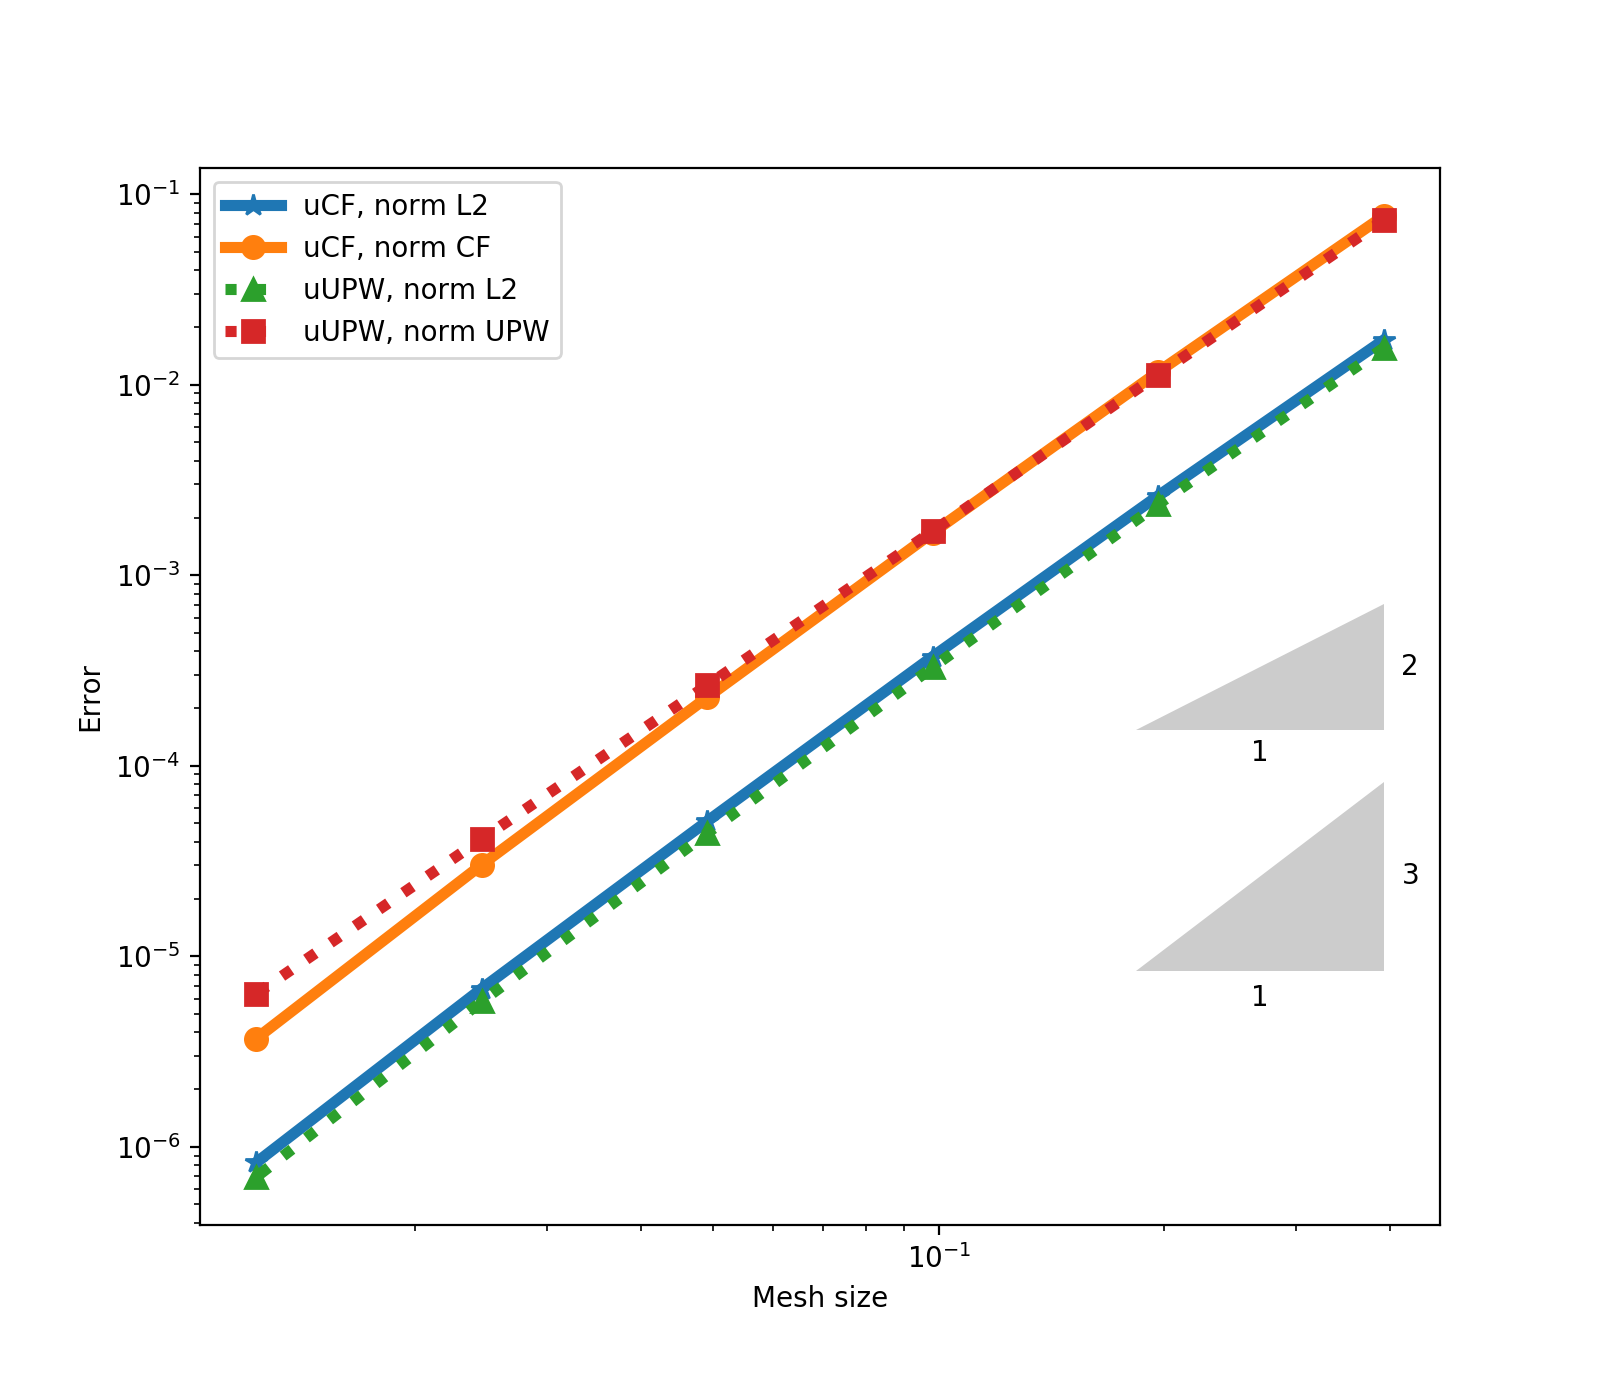
\includegraphics[scale=0.30]{img/Conveccion_Reaccion/errores_conveccion_reaccion_P2dc.png}
			\captionof{figure}{Errores en escala logarítmica.}
		\end{minipage}
		\end{frame}

\begin{frame}{References}
	\scriptsize 
	\vspace*{-0.25cm}
	\nocite*
	\bibliographystyle{apalike}
	\bibliography{references}
\end{frame}

\begin{frame}{}
	\centering
	\vspace*{1cm}
	{\Huge
		\emph{Thanks for your attention!}}
	
	\vspace*{0.5cm}
	\emph{Happy birthday Giuseppe!}
	
	\vspace*{1cm}
	\begin{acknowledgements}
		The speaker has been supported by a \textit{Graduate Scholarship funded by the University of Tennessee at Chattanooga}; by \textit{UCA FPU contract UCA/REC14VPCT/2020, Erasmus+ KA131 and travel grants funded by Universidad de Cádiz}.
		
		The collaborators have been supported by \textit{Grant US-4931381261 (US/JUNTA/FEDER, UE)}.
	\end{acknowledgements}
\end{frame}